% Options for packages loaded elsewhere
\PassOptionsToPackage{unicode}{hyperref}
\PassOptionsToPackage{hyphens}{url}
\PassOptionsToPackage{dvipsnames,svgnames,x11names}{xcolor}
%
\documentclass[
  singlecolumn,
  9pt]{article}

\usepackage{amsmath,amssymb}
\usepackage{iftex}
\ifPDFTeX
  \usepackage[T1]{fontenc}
  \usepackage[utf8]{inputenc}
  \usepackage{textcomp} % provide euro and other symbols
\else % if luatex or xetex
  \usepackage{unicode-math}
  \defaultfontfeatures{Scale=MatchLowercase}
  \defaultfontfeatures[\rmfamily]{Ligatures=TeX,Scale=1}
\fi
\usepackage[]{libertinus}
\ifPDFTeX\else  
    % xetex/luatex font selection
\fi
% Use upquote if available, for straight quotes in verbatim environments
\IfFileExists{upquote.sty}{\usepackage{upquote}}{}
\IfFileExists{microtype.sty}{% use microtype if available
  \usepackage[]{microtype}
  \UseMicrotypeSet[protrusion]{basicmath} % disable protrusion for tt fonts
}{}
\makeatletter
\@ifundefined{KOMAClassName}{% if non-KOMA class
  \IfFileExists{parskip.sty}{%
    \usepackage{parskip}
  }{% else
    \setlength{\parindent}{0pt}
    \setlength{\parskip}{6pt plus 2pt minus 1pt}}
}{% if KOMA class
  \KOMAoptions{parskip=half}}
\makeatother
\usepackage{xcolor}
\usepackage[top=30mm,bottom=30mm,left=20mm,heightrounded]{geometry}
\setlength{\emergencystretch}{3em} % prevent overfull lines
\setcounter{secnumdepth}{-\maxdimen} % remove section numbering
% Make \paragraph and \subparagraph free-standing
\ifx\paragraph\undefined\else
  \let\oldparagraph\paragraph
  \renewcommand{\paragraph}[1]{\oldparagraph{#1}\mbox{}}
\fi
\ifx\subparagraph\undefined\else
  \let\oldsubparagraph\subparagraph
  \renewcommand{\subparagraph}[1]{\oldsubparagraph{#1}\mbox{}}
\fi


\providecommand{\tightlist}{%
  \setlength{\itemsep}{0pt}\setlength{\parskip}{0pt}}\usepackage{longtable,booktabs,array}
\usepackage{calc} % for calculating minipage widths
% Correct order of tables after \paragraph or \subparagraph
\usepackage{etoolbox}
\makeatletter
\patchcmd\longtable{\par}{\if@noskipsec\mbox{}\fi\par}{}{}
\makeatother
% Allow footnotes in longtable head/foot
\IfFileExists{footnotehyper.sty}{\usepackage{footnotehyper}}{\usepackage{footnote}}
\makesavenoteenv{longtable}
\usepackage{graphicx}
\makeatletter
\def\maxwidth{\ifdim\Gin@nat@width>\linewidth\linewidth\else\Gin@nat@width\fi}
\def\maxheight{\ifdim\Gin@nat@height>\textheight\textheight\else\Gin@nat@height\fi}
\makeatother
% Scale images if necessary, so that they will not overflow the page
% margins by default, and it is still possible to overwrite the defaults
% using explicit options in \includegraphics[width, height, ...]{}
\setkeys{Gin}{width=\maxwidth,height=\maxheight,keepaspectratio}
% Set default figure placement to htbp
\makeatletter
\def\fps@figure{htbp}
\makeatother
% definitions for citeproc citations
\NewDocumentCommand\citeproctext{}{}
\NewDocumentCommand\citeproc{mm}{%
  \begingroup\def\citeproctext{#2}\cite{#1}\endgroup}
% avoid brackets around text for \cite:
\makeatletter
 \def\@biblabel#1{}
 \def\@cite#1#2{{#1\if@tempswa , #2\fi}}
\makeatother
\newlength{\cslhangindent}
\setlength{\cslhangindent}{1.5em}
\newlength{\csllabelwidth}
\setlength{\csllabelwidth}{3em}
\newlength{\cslentryspacing}
\setlength{\cslentryspacing}{0em}
\usepackage{enumitem}
\newlist{CSLReferences}{itemize}{1}
\setlist[CSLReferences]{label={},
  leftmargin=\cslhangindent,
  itemindent=-1\cslhangindent,
  parsep=\parskip,
  itemsep=\cslentryspacing}
\usepackage{calc}
\newcommand{\CSLBlock}[1]{#1\hfill\break}
\newcommand{\CSLLeftMargin}[1]{\parbox[t]{\csllabelwidth}{#1}}
\newcommand{\CSLRightInline}[1]{\parbox[t]{\linewidth - \csllabelwidth}{#1}\break}
\newcommand{\CSLIndent}[1]{\hspace{\cslhangindent}#1}

\usepackage{cancel}
\usepackage[noblocks]{authblk}
\renewcommand*{\Authsep}{, }
\renewcommand*{\Authand}{, }
\renewcommand*{\Authands}{, }
\renewcommand\Affilfont{\small}
\usepackage{cancel}
\makeatletter
\makeatother
\makeatletter
\makeatother
\makeatletter
\@ifpackageloaded{caption}{}{\usepackage{caption}}
\AtBeginDocument{%
\ifdefined\contentsname
  \renewcommand*\contentsname{Table of contents}
\else
  \newcommand\contentsname{Table of contents}
\fi
\ifdefined\listfigurename
  \renewcommand*\listfigurename{List of Figures}
\else
  \newcommand\listfigurename{List of Figures}
\fi
\ifdefined\listtablename
  \renewcommand*\listtablename{List of Tables}
\else
  \newcommand\listtablename{List of Tables}
\fi
\ifdefined\figurename
  \renewcommand*\figurename{Figure}
\else
  \newcommand\figurename{Figure}
\fi
\ifdefined\tablename
  \renewcommand*\tablename{Table}
\else
  \newcommand\tablename{Table}
\fi
}
\@ifpackageloaded{float}{}{\usepackage{float}}
\floatstyle{ruled}
\@ifundefined{c@chapter}{\newfloat{codelisting}{h}{lop}}{\newfloat{codelisting}{h}{lop}[chapter]}
\floatname{codelisting}{Listing}
\newcommand*\listoflistings{\listof{codelisting}{List of Listings}}
\makeatother
\makeatletter
\@ifpackageloaded{caption}{}{\usepackage{caption}}
\@ifpackageloaded{subcaption}{}{\usepackage{subcaption}}
\makeatother
\makeatletter
\makeatother
\ifLuaTeX
  \usepackage{selnolig}  % disable illegal ligatures
\fi
\IfFileExists{bookmark.sty}{\usepackage{bookmark}}{\usepackage{hyperref}}
\IfFileExists{xurl.sty}{\usepackage{xurl}}{} % add URL line breaks if available
\urlstyle{same} % disable monospaced font for URLs
\hypersetup{
  pdftitle={Causal Diagrams for the Evolutionary Human Sciences: A Practical Guide},
  pdfauthor={Joseph A. Bulbulia},
  pdfkeywords={Directed Acyclic Graph, Causal
Inference, Confounding, Feedback, Interaction, Mediation, Moderation, Panel},
  colorlinks=true,
  linkcolor={blue},
  filecolor={Maroon},
  citecolor={Blue},
  urlcolor={Blue},
  pdfcreator={LaTeX via pandoc}}

\title{Causal Diagrams for the Evolutionary Human Sciences: A Practical
Guide}


  \author{Joseph A. Bulbulia}
            \affil{%
                  Victoria University of Wellington, New Zealand, School
                  of Psychology, Centre for Applied Cross-Cultural
                  Research
              }
      
\date{2023-11-25}
\begin{document}
\maketitle
\begin{abstract}
This article offers practical advice for creating causal diagrams. It
recommends aligning a graph's spatial layout with causation's temporal
order. Because causal graphs only have utility within the framework of
theories and assumptions that define causal data science, I begin by
reviewing this framework. I then consider how, within this framework,
causal diagrams may be used to uncover structural sources of bias. I
focus on confounding bias, and illustrate the benefits of chronological
hygiene in one's graph, not only for data analysis but also for data
collection. I conclude by using causal diagrams to elucidate the widely
misunderstood concepts causal interaction, mediation, and dynamic
longitudinal feedback, again focussing on the benefits of chronological
ordering for data analysis and collection. Overall, this guide hopes to
better equip evolutionary human scientists with understanding and skills
to enhance the rigour and clarity of their causal inferences.
\end{abstract}
\subsection{Introduction}\label{introduction}

Correlation does not imply causation. This adage is widely known.
Nevertheless, many human scientists report manifest correlations and use
hedging language that implies causation. I have been guilty. However,
such reporting typically lacks justification. Making matters worse,
widely adopted strategies for confounding control such as indiscriminate
co-variate adjustment are known to enhance bias
(\citeproc{ref-mcelreath2020}{McElreath 2020}). Across many human
sciences, including the evolutionary human sciences, persistent
confusion in the analysis and reporting of correlations has greatly
impeded scientific progress, what might be described as a `causality
crisis' (\citeproc{ref-bulbulia2022}{Bulbulia 2022}).

There is hope. First, the open science movement has demonstrated that
greater attention to the `replication crisis' in the experimental human
sciences can bring considerable improvements within a relatively short
span of time. Although much remains to be done still, many corrective
practices in open science have become normative. Second, several decades
of development in causal data science in the health sciences, computer
sciences, economics, and some social sciences have yielded both
considerable conceptual clarifications and rigorous analytic toolkits
for inference (\citeproc{ref-hernan2023}{Hernan and Robins 2023};
\citeproc{ref-neyman1923}{Neyman 1923}; \citeproc{ref-pearl2009a}{Pearl
2009b}; \citeproc{ref-pearl1995}{Pearl and Robins 1995a};
\citeproc{ref-robins1986}{Robins 1986}; \citeproc{ref-rubin1976}{Rubin
1976}; \citeproc{ref-vanderweele2015}{VanderWeele 2015}). Although
causal data science is still evolving (\citeproc{ref-duxedaz2021}{Díaz
\emph{et al.} 2021}; \citeproc{ref-hoffman2023}{Hoffman \emph{et al.}
2023}; \citeproc{ref-vansteelandt2022}{Vansteelandt and Dukes 2022}) , a
substantial foundation for causal data science already exists. Given
these precedents, we should be optimistic that rapid uptake of causal
data science in those fields where causal confusion currently holds sway
is a feasible and achievable goal. The articles in this special issue of
\emph{Evolutionary Human Sciences} offer testimony to this hope.

Causal diagrams, also known as `directed acyclic graphs' or `DAGs,' are
powerful inferential tools in the workflows of causal data science.
These tools rest on a robust system of formal mathematical proofs,
instilling confidence in their use. However, they do not require
mathematical training. As such, causal diagrams are broadly accessible,
for the sighted. However, causal diagrams only acquire their
significance when integrated within the broader theoretical frameworks
causal data science, which distinguishes itself from traditional data
science by attempting to estimate pre-specified counterfactual
contrasts, or `estimands'. In this approach, counterfactual scenarios
are simulated from data under explicit expert assumptions and then
quantitatively compared. Causal Data Science can be viewed as a form of
`counterfactual data science' or `full data science' --- `full' in the
sense that the data we observe provide only partial insights into the
targeted causal quantities and uncertainties researchers hope to
consistently estimate (reference: (\citeproc{ref-bulbulia2023}{Bulbulia
2023}); see also: (\citeproc{ref-ogburn2021}{Ogburn and Shpitser
2021})). Using causal diagrams without a thorough understanding of their
role in Causal Data Science risks inadvertently worsen the causality
crisis by fostering misguided confidence where none is due.

In this work, I aim to offer readers of \emph{Evolutionary Human
Science} practical guidance on creating causal diagrams in ways that
mitigate the risk of overreaching.

\textbf{Part 1} introduces the core elements of Causal Data Science,
emphasising the fundamental assumptions necessary for obtaining valid
causal inferences from observational data. Although this overview is
brief, it is vital for researchers using causal diagrams to familiarise
themselves with these foundational concepts (see also other references
in this issue), and to understand the place of causal diagrams within
wider systematic workflows.

\textbf{Part 2} introduces \textbf{chronologically ordered causal
diagrams} and their applications in addressing confounding bias. We
discover that maintaining chronological order in the spatial layout of
these diagrams clarifies structural biases, enhances strategies for
identifying causal effect estimates, and indicates where causal
inferences may remain elusive. Chronologically ordered causal diagrams
also underscore the value of collecting repeated measures over time,
thereby improving research planning. Although, chronological ordering is
not strictly essential for the utility of a causal diagram, the examples
we consider demonstrate their advantages in common scenarios.

\textbf{Part 3} uses chronologically ordered causal diagrams to
demystify complex concepts such as causal interaction, mediation, and
longitudinal data analysis. Here, attention to chronological sequencing
in the diagram's layout scientific comprehension. This approach enables
us to more effectively formulate and address causal questions in areas
where standard data science traditions such structural equation
modelling continue to perpetuate confusions. We again observe that
attention to chronological hygiene enhances the transparency of the
analysis and, even equally fundamental, directs focus on absolute
requirements for ensuring clear measurements for the timing of events in
data collection.

There are numerous excellent resources available for learning causal
diagrams, which I highly recommend to readers
(\citeproc{ref-barrett2021}{Barrett 2021};
\citeproc{ref-cinelli2022}{Cinelli \emph{et al.} 2022};
\citeproc{ref-greenland1999}{Greenland \emph{et al.} 1999a};
\citeproc{ref-hernuxe1n2023}{Hernán and Monge 2023};
\citeproc{ref-mcelreath2020}{McElreath 2020};
\citeproc{ref-pearl2009}{Pearl 2009a}; \citeproc{ref-rohrer2018}{Rohrer
2018}; \citeproc{ref-suzuki2020}{Suzuki \emph{et al.}
2020a}).\footnote{An excellent resource is Miguel Hernán's free online
  course, here:
  \url{https://pll.harvard.edu/course/causal-diagrams-draw-your-assumptions-your-conclusions}.}
Here, I build on this this work by providing additional conceptual
orientation to the frameworks of Causal Data Science in which causal
diagrams have their place, and by underscoring the importance of
chronological hygiene for pinpointing structural sources of confounding
bias and for ensuring accurate timing of the sequence of events recorded
in researchers datasets. Finally, this guide integrates the knowledge
about the frameworks of Causal Data Science with chronologically ordered
causal diagrams to shed light on the concepts of interaction, mediation,
and longitudinal feedback, about which there remains considerable
confusion in the sub-fields that inform the evolutionary human sciences,
particularly those that developed under the influence of structural
equation modelling.

\subsection{Part 1. Overview of Causal Data
Science}\label{part-1.-overview-of-causal-data-science}

The critical first step in causal inference is to formulate a
well-defined causal question (\citeproc{ref-hernuxe1n2016}{Hernán
\emph{et al.} 2016}). First, we must consider the specific treatments or
interventions of interest, the specific outcomes we seek to contrast and
their timing, the scale on which the causal contrasts will be made, and
the populations of units to which we hope our inferences to generalise.
Causal diagrams come later, as we consider which forms of data might
enable us to address our pre-specified causal questions. This section
introduces fundamental concepts in Causal Data Science, and locates the
place of causal diagrams within a larger workflow that moves from
stating a causal question to answering it with data.

\subsubsection{The Fundamental Problem of Causal
Inference}\label{the-fundamental-problem-of-causal-inference}

Consider an intervention, \(A\), and its effect, \(Y\). We say that
\(A\) causes \(Y\) if altering \(A\) would lead to a change in \(Y\)
(\citeproc{ref-hume1902}{Hume 1902}; \citeproc{ref-lewis1973}{Lewis
1973}). If altering \(A\) would not lead to a change in \(Y\), then we
say that \(A\) has no causal effect on \(Y\).

The objective in causal inference is to measure obtain a contrast at
some scale, such as the difference scale, in a well-defined outcome
\(Y\) when subjected to different levels of a well-defined intervention
\(A\). Commonly, we refer to such interventions as `exposures' or
`treatments;' we refer to the possible effects of interventions as
`potential outcomes.'

Let us assume that \(A\) exists in two states: \(A = 0\) or \(A = 1\).
We denote the potential outcome when \(A\) is set to \(0\) as \(Y(0)\)
and when \(A\) is set to 1 as \(Y(1)\).\footnote{There are different
  conventions for representing potential outcomes under different
  interventions, such as \(Y^a\) and \(Y_a\). To simplify, except where
  context demands clarity, we omit subscripts, using for example
  \(Y(1) - Y(0)\) in place of \(Y_i(1) - Y_i(0)\) when indexing causal
  effects to an individual. We follow this convention for realised
  outcomes, preferring \(Y|A = 0\) or \(Y|A = 1\) to \(Y_i|A_i = 0\) or
  \(Y_i|A_i = 1\), except when clarity demands. Additionally, except
  when clarity demands, we omit the implicit time subscripts; for a time
  index \(t\), allowing our simplified convention to stand in place of
  \(Y_{i,t+1}|A_{i,t} = 0\) and \(Y_{i,t+1}|A_{i,t} = 1\). We employ
  this simplified notation for legibility, and, when discussing
  potential outcomes, for accuracy. Potential outcomes are not random
  realisations of distribution but rather fixed features of reality, see
  (\citeproc{ref-hernan2023}{Hernan and Robins 2023 p. 6} note). To
  invoke the \emph{Wizard of Oz}, Causal Data Science does not begin its
  journey in the ``Kansas'' of ordinary statistical science. It rather
  begins its journey in a counterfactual OZ. The meaning of this
  reference will become concrete below. Indeed any who have conducted
  experiments will be familiar with it.}

At any given moment, for any unit under consideration, only one level of
an exposure can be realised. Consider hypothetical questions such as
`What if Isaac Newton had not observed the falling apple?' or `What if
Leonardo da Vinci had never pursued art?' or `What if Archduke Ferdinand
had not been assassinated?' Unfortunately, we cannot observe what would
have happened had history been different. The physics of middle-sized
dry goods that applies to persons and cultures prevents this. History is
characterised by a unidirectional progression. Suppose we have specified
a well-defined exposure and outcome. Each unit can either experience
\(Y|A = 1\) or \(Y|A = 0\), but never both simultaneously. As a result,
we cannot directly calculate a contrast between \(Y(1)\) and \(Y(0)\)
from our available data. In every case, at least one of the outcomes
necessary to determine a causal effect at the individual level remains
counterfactual. The inaccessibility of at least one of the potential
outcomes we require to compute a causal contrast from data is known as
the `fundamental problem of causal inference'
(\citeproc{ref-holland1986}{Holland 1986};
\citeproc{ref-rubin1976}{Rubin 1976}). What applies to one unit applies
to all units. Causal data science faces a unique type of missing data
problem in which the `full data' needed to compute any causal contrast
is missing at least half of its values
(\citeproc{ref-edwards2015}{Edwards \emph{et al.} 2015};
\citeproc{ref-westreich2015}{Westreich \emph{et al.} 2015}). This
challenge is distinct from typical missing data scenarios where data
could have been recorded but were not. The missing information crucial
for computing causal contrasts is intrinsically linked to the
irreversible nature of time.

\subsubsection{Obtaining Average Causal Effects From
Observations}\label{obtaining-average-causal-effects-from-observations}

In typical scenarios, computing individual causal effects is not
feasible. However, under certain assumptions, it is possible to credibly
calculate average causal effects. That is, we may obtain average
treatment effects by contrasting groups that have received different
levels of a treatment. The average treatment effect (ATE) on a
difference scale is represented as:

\[
ATE  = \mathbb{E}[Y(1)] - \mathbb{E}[Y(0)]
\]

Here, \(\mathbb{E}\) denotes the average response of all individuals
within an exposure group, and \(Y(1)\) and \(Y(0)\) represent the
potential outcomes under interventions \(A = 1\) and \(A = 0\),
respectively.

How might we obtain average causal effects when individual causal
effects are not observable? It is helpful to consider how randomised
experiments obtain such contrasts.

First, let us state the problem in terms of the `full data' we would
need were we to base these contrasts on observations. Where ATE denotes
the ``Average Treatment Effect'':

\[
ATE = \left(\underbrace{\underbrace{\mathbb{E}[Y(1)|A = 1]}_{\text{observed for } A = 1} + \underbrace{\mathbb{E}[Y(1)|A = 0]}_{\text{unobserved for } A = 0}}_{\text{effect among treated}}\right) - \left(\underbrace{\underbrace{\mathbb{E}[Y(0)|A = 0]}_{\text{observed for } A = 0} + \underbrace{\mathbb{E}[Y(0)|A = 1]}_{\text{unobserved for } A = 1}}_{\text{effect among untreated}}\right)
\]

In each treatment condition, we do not observe the potential outcome for
every unit that did not receive the opposite level of treatment they in
fact received. However, when researchers randomise units into treatments
conditions, then the distribution of variables that might affect each
potential outcome independently of the exposure cancel each other out
when averaging over the groups. When treatments are randomly assigned,
and randomisation is effective, the outcomes under different treatment
conditions should, in theory, be identical on average.

\[
 E[Y(0) | A = 1] = E[Y(0) | A = 0] 
\]

\[
E[Y(1) | A = 1] = E[Y(1) | A = 0] 
\]

And thus,

\[
  \widehat{ATE} = \mathbb{E}[Y | A = 1] - \mathbb{E}[Y | A = 0]
\]

Where \(\widehat{ATE}\) is the predicted average treatment effect.

Although randomisation can fail, it provides a means to identify
group-level causal effects by eliminating other potential explanations
for the observed differences. Like Sherlock Holmes, any observed
difference between the treatment groups may be attributable to the
treatment because successful randomisation exhausts every other
explanation. By randomisation, the distribution of potential outcomes is
the same across treatment groups. For this reason, we should prefer
experiments for addressing scientific questions that can be addressed by
them.

Regrettably, many scientific questions, particularly those in the
evolutionary human sciences, cannot be addressed through experimental
means. This limitation is acutely felt when researchers confront `what
if?' scenarios rooted in the unidirectional nature of human history.
However, understanding how radomisation obtains missing counterfactual
outcomes clarifies the tasks of causal data science in observational
settings (\citeproc{ref-hernuxe1n2008a}{Hernán \emph{et al.} 2008};
\citeproc{ref-hernuxe1n2022}{Hernán \emph{et al.} 2022a};
\citeproc{ref-hernuxe1n2006}{Hernán and Robins 2006}). We must obtain
balance across variables that might account for treatment-level
differences. This task presents a significant challenge. Observations
typically cannot in themselves verify no-unmeasured confounding.
Moreover, we must satisfy ourselves of additional assumptions, which are
nearly automatic in randomised experimental settings but which cannot be
taken for granted elsewhere. We group these assumption into two
categories: (1) Fundamental identification assumptions; (2) Data and
modelling assumptions. We next consider these assumptions, clarifying
where in the workflow causal diagrams help causal data scientists to
satisfy them.

\subsubsection{Fundamental Identification
Assumptions}\label{fundamental-identification-assumptions}

There are three fundamental identification assumptions that must be
satisfied to estimate causal effects with data.

\paragraph{Fundamental Identification Assumption 1: Causal Consistency
and Treatment Effect
Heterogeneity}\label{fundamental-identification-assumption-1-causal-consistency-and-treatment-effect-heterogeneity}

The causal consistency assumption posits that for any given level of
exposure, \(A=a\), the observed outcome, \(Y|A=a\), is interchangeable
with the counterfactual outcome: \(Y(a)|A = a\). To illustrate, we will
use the subscript \(i\) to represent an individual. The observed outcome
when treatment is \(A_i = a\) is denoted as \(Y_i^{observed}|A_i = a\).
When the causal consistency assumption is satisfied, the observed
outcome for each individual \(i...N\) corresponds to one of the
counterfactual outcomes necessary for calculating a causal contrast:

\[
Y_i^{observed}|A_i = 
\begin{cases} 
Y_i(a^*) & \text{if } A_i = a^* \\
Y_i(a) & \text{if } A_i = a
\end{cases}
\]

This assumption implies that the observed outcome at a specific exposure
level mirrors the counterfactual outcome for that individual. Although
it might seem straightforward to equate an individual's observed outcome
with their counterfactual outcome, in observational studies, treatment
effects often vary, posing considerable challenges in satisfying this
assumption.

Consider the question of whether a society's beliefs in Big Gods affects
its development of Social Complexity {[}CITE{]}. Historians and
anthropologists report that such beliefs vary over time and across
cultures in their intensity, interpretations, institutional management,
and ritual embodiments {[}CITE{]}. Such variation in content and setting
may significantly influence social complexity. Moreover the treatments
as they are realised in one society might affect the treatments realised
in other societies. Often, it may be unclear how we can address the
treatment independence assumption using a conditioning strategy. I
review additional problems in Appendix 1. For now, the manifest
variation in treatments we should assume to hold in this setting
underscores the need for careful consideration whether \emph{treatment
heterogeneity} allows us to assume conditional exchangeability.

The theory of causal inference under multiple versions of treatment,
developed by VanderWeele and Hernán, formally addresses the challenge of
treatment heterogeneity (\citeproc{ref-vanderweele2009}{VanderWeele
2009a}, \citeproc{ref-vanderweele2018}{2018};
\citeproc{ref-vanderweele2013}{VanderWeele and Hernan 2013}). The
authors proved that if the treatment variations (\(K\)) are
conditionally independent of the outcome \(Y(k)\) given covariates
\(L\), then conditioning on \(L\) allows us to consistently estimate a
causal contrast over the heterogeneous treatments.

Where \(\coprod\) denotes independence, causal consistency is formally
preserved if

\[
K \coprod Y(k) | L
\]

Under the theory of causal inference under multiple versions of
treatment, we think of \(K\) as a ``coarsened indicator'' for \(A\).
That is, we obtain an average effect estimate for the multiple treatment
versions \(K\) on \(Y(k)\).

Although the theory of causal inference under multiple versions of
treatment provides a formal solution to the problem of treatment effect
heterogeneity, interpreting the resulting causal effect estimates under
this theory can be challenging. Consider the question of whether Body
Mass Index (BMI) affects health (\citeproc{ref-hernuxe1n2008}{Hernán and
Taubman 2008}). Notably, weight loss can occur through various methods,
each with different health implications. Some methods, such as regular
exercise or a calorie-reduced diet, are generally beneficial for health.
However, weight loss might also result from adverse conditions such as
infectious diseases, cancers, depression, famine, or even amputations,
which are not beneficial to health. Although causal effects can be
consistently estimated while adjusting for covariates \(L\), the true
nature and implications of the changes in BMI might remain unclear. This
uncertainty highlights the need for precise and well-defined causal
questions. For example, rather than stating the intervention as
``weightloss'', we state the intervention as weight loss achieved
specifically through aerobic exercise over a period of at least five
years, compared with no weight loss. This level of specificity in our
exposure and outcomes helps ensure that the causal estimates we obtain
are not only statistically sound but also interpretable (for discussion
see: (\citeproc{ref-hernuxe1n2022a}{Hernán \emph{et al.} 2022b};
\citeproc{ref-hernuxe1n2008}{Hernán and Taubman 2008};
\citeproc{ref-murray2021a}{Murray \emph{et al.} 2021}).

Beyond interpretation, there is the additional problem that we cannot
really know whether the measured covariates \(L\) suffice to render the
multiple-versions of treatment independent of the counterfactual
outcomes. This problem is especially acute when there are spill-over
effects, such when treatment-effects are relative to the density and
distribution of treatment-effects in a population {[}CITE{]}. For this
reason, causal data science must rely heavily on sensitivity analyses
(VanderWeele (\citeproc{ref-vanderweele2019}{2019});).

Thus, what seemed initially to be a near truism -- that each units
observed outcome may be assumed to correspond to that unit's
counterfactual outcome -- turns out to be a strong assumption. In many
settings, causal consistency should be presumed unrealistic until proven
tenable. For now, we note that the causal consistency assumption
provides a theoretical starting point for recovering the missing
counterfactuals essential for computing causal contrasts. It achieves
this by identifying half of these counterfactuals directly from observed
data. The concept of exchangeability, which we will explore next, offers
a means to derive the remaining half of the missing counterfactuals we
require to consistently compute causal contrasts.

\paragraph{Fundamental Identification Assumption 2: Conditional
Exchangeability (No Unmeasured
Confounding)}\label{fundamental-identification-assumption-2-conditional-exchangeability-no-unmeasured-confounding}

We satisfy conditional exchangeability when the treatment groups are
equivalent in variables that could affect potential outcomes. In
experimental designs, random assignment facilitates conditional
exchangeability. In observational studies, more effort is required. We
must control for covariates that could account for observed correlations
between \(A\) and \(Y\) in the absence of a causal effect of \(A\) on
\(Y\) for every observed.

Let \(L\) denote the set of covariates necessary to ensure this
conditional independence. Let \(\coprod\) again denote independence. We
satisfy conditional exchangeability when:

\[
Y(a) \coprod A | L \quad \text{or equivalently} \quad A \coprod Y(a) | L
\]

Where this, and the other fundamental assumptions hold, we may compute
the average treatment effect (ATE) on the difference scale:

\[
ATE = \mathbb{E}[Y(a^*) | L] - \mathbb{E}[Y(a) | L]
\]

In the disciplines of cultural evolution, where experimental control is
often impractical, causal inferences hinge on the plausibility of
satisfying this `no unmeasured confounding' assumption. Lacking
randomisation, however, causal data science must turn to sensitivity
analyses (Appendix 1 critiques such assumptions for estimating causal
effects of beliefs in Big Gods on social complexity).

Importantly, \emph{the primary purpose of a causal diagram within a
causal inference workflow is to evaluate the conditional exchangeability
assumption.} Causal diagrams enable researchers to represent crucial
structural assumptions that are necessary for achieving balance in the
confounders across levels of the exposure stated in a pre-specified
causal contrast.

Moreover, it is important to recognise that in this setting, causal
diagrams are designed to \emph{highlight only those aspects the assumed
causal order pertinent to the assessment of `no-unmeasured
confounding.'} A common mistake when creating a causal diagram is to
provide too much detail, obscuring rather than clarifying structural
sources of bias. Please keep your graph minimal.

\paragraph{Fundamental Identification Assumption 3:
Positivity}\label{fundamental-identification-assumption-3-positivity}

We may say the positivity assumption is met when there exists a non-zero
probability for each level of exposure within every level of covariates
needed to ensure conditional exchangeability. This implies that for each
stratification of every covariate, the probability that for each level
of exposure value must exceed zero. Where \(A\) is the exposure and
\(L\) a vector of covariates, positivity is only achieved if

\[
0 < \Pr(A = a | L = l) < 1, ~ \forall a \in A, ~ \forall l \in L
\]

There are two types of positivity violation:

\begin{enumerate}
\def\labelenumi{\arabic{enumi}.}
\item
  \textbf{Random non-positivity:} which occurs when an exposure is
  theoretically possible, but specific exposure levels are not
  represented in the data. Notably, random non-positivity is the only
  identifiability assumption verifiable with data.
\item
  \textbf{Deterministic non-positivity:} which occurs when the exposure
  is implausible by nature. For instance, a hysterectomy in biological
  males would appear biologically implausible.
\end{enumerate}

Satisfying the positivity assumption may present considerable data
challenges within the workflows of causal data science
(\citeproc{ref-westreich2010}{Westreich and Cole 2010}). Consider
estimating the effects of church attendance on charity. Suppose our
objective is to assess the one-year effect on charitable donations
following a shift from no church attendance to weekly attendance. Assume
we have access to extensive panel data that has tracked 20,000
individuals over three years. Consider, the natural transition rate from
no attendance to weekly attendance in many human populations will be
quite low. Suppose it is one in a thousand annually. In that case, the
effective sample for the treatment condition dwindles to 20. Despite
abundant data, attention to the positivity assumptions reveals the data
required for valid contrasts is sparse.

Note that where positivity is violated, causal diagrams offer limited
assistance to causal inference because causal inference is not supported
by the data.

\subsubsection{Practical Considerations}\label{practical-considerations}

Beyond the three fundamental identification assumptions that must be
satisfied to estimate causal effects with data, there are numerous
practical consideration that enter into any causal inference workflow.

\paragraph{Overly ambitious estimands}\label{overly-ambitious-estimands}

In causal inference, the notion of assessing Average Treatment Effects
(ATE) through \(E[Y(1) - Y(0)|L]\) is often flawed, particularly in the
context of continuous exposures. This approach simplifies the complexity
of real-world phenomena by forcing a binary framework on continuous
variables, which is inherently problematic. For example, categorising
continuous exposures into quartiles and comparing, say, the lowest with
the third quartile, grossly oversimplifies the phenomena under study.
This method not only stretches the positivity assumption to its breaking
point, but it also frequently breaches it. The real-world simply does
not operate in such neatly defined exposure levels, rendering these
comparisons artificial and potentially misleading.

Moreover, the assumption of a monotonic relationship between treatment
and effect is equally naive. Real-life treatment effects are rarely
linear or straightforward. By comparing arbitrary points on a continuous
scale, we risk drawing erroneous conclusions about the treatment's
overall impact. This approach is a shortcut that distorts the true
nature of the treatments effect.

Focusing on ATE also masks the vital heterogeneity in treatment effects.
This heterogeneity is not just a statistical nuisance; it is the essence
of understanding causal mechanisms. Average effects blur the variations
and nuances that are critical for informed decision-making. Recognising
and elucidating this heterogeneity should be a primary goal, yet current
methods fall short. The field is evolving (see: Tchetgen and VanderWeele
(\citeproc{ref-tchetgen2012}{2012}); Wager and Athey
(\citeproc{ref-wager2018}{2018}); Cui \emph{et al.}
(\citeproc{ref-cui2020}{2020}), Vansteelandt and Dukes
(\citeproc{ref-vansteelandt2022}{2022})). These emerging methodologies,
while promising, are still in their infancy and are not yet capable of
fully addressing the complex nature of heterogeneous treatment effects
in continuous exposure settings. Such limitations must be clarified at
the outset of inquiry.

\paragraph{Consideration of measurement error
bias}\label{consideration-of-measurement-error-bias}

Measurement error refers to the discrepancy between the true value of a
variable and the value that is observed or recorded. This error can
arise from a variety of sources, including instrument calibration,
respondent misreporting, or coding errors. Unfortunately, measurement
error is both commonplace, and capable of significantly distorting
causal inferences.

Briefly, measurement error confounding can be classified into two main
types: systematic (directed) and uncorrelated (undirected).

\textbf{Systematic measurement error:} occurs when the measurements
deviate from the true value in a consistent direction. Systematic errors
can lead to biased estimates of causal effects, as they consistently
overestimate or underestimate true causal magnitudes.

\textbf{Random measurement error:} occurs when fluctuations in the
measurement process and do not consistently bias the data in one
direction. While random measurement errors can increase the variability
of data and reduce statistical power, they do not typically introduce
bias in estimates of causal effects when there are no such effects.
However, random measurement error can attenuate bias when there are true
causal effects, where the estimated effect of an exposure on an outcome
is systematically weakened.

To handle measurement error the best approach is to improving data
quality; this is not always possible, and so we must perform sensitivity
analyses.

Causal diagrams may be powerful aids for evaluating structural sources
of bias that may arise from different forms of measurement error
(\citeproc{ref-hernan2023}{Hernan and Robins 2023};
\citeproc{ref-hernuxe1n2009}{Hernán and Cole 2009};
\citeproc{ref-vanderweele2012a}{VanderWeele and Hernán 2012}). We will
not consider this use here {[}CITE OTHER PAPER{]}. For now, it is
important to emphasise that the simple causal diagrams with arrows
between variables typically abstract away from biases that arise from
measurement error, and such simplicity can be a source of false
confidence.\footnote{The careful reader will note a tension. Addressing
  structural sources of bias requires simple causal diagrams. Such
  diagrams do not capture the threats to inference arising from
  measurement, which requires more complicated causal diagrams. Hernán
  and Robins advise a two step approach in which authors draft separate
  diagrams to handle separate threats to valid causal inference
  (\citeproc{ref-hernuxe1n2023}{Hernán and Monge 2023}).}

\paragraph{Consideration of selection
bias}\label{consideration-of-selection-bias}

Selection bias arises when the sample that is observed is not
representative of the population for which causal inference is intended.
There are two primary forms: bias arising to initial selection and bias
resulting from attrition or non-response
(\citeproc{ref-bareinboim2022a}{Bareinboim \emph{et al.} 2022};
\citeproc{ref-hernuxe1n2004a}{Hernán \emph{et al.} 2004};
\citeproc{ref-hernuxe1n2017}{Hernán 2017}; \citeproc{ref-lu2022}{Lu
\emph{et al.} 2022}; \citeproc{ref-suzuki2020a}{Suzuki \emph{et al.}
2020b}).\footnote{It is important to note that the term ``selection on
  observables'' is used differently in economics compared to
  epidemiology and public health, as I am using the term here. In
  economics, ``selection on observables'' typically refers to the
  non-random treatment assignments in observational data. In this
  context, if all variables that influence both the selection process
  and the outcome are observed and accounted for, the resulting bias can
  be controlled for in the analysis. Terminological differences abound
  in casual data science. It is crucial to be aware of these
  distinctions and clarify the specific usage within the context of
  one's study to avoid confusion and ensure accurate communication.}

\textbf{Selection prior to observation:} the bias when the process of
selecting individuals or units for the study leads to a
non-representative sample of the target population. This bias may arise
from specific inclusion or exclusion criteria or through non-random
selection methods. Such bias can introduce systematic differences
between treatment and control groups, affecting the generalizability of
results. Consequently, the estimates obtained might not accurately
reflect the causal effects in the intended population.

\textbf{Attrition/non-response bias:} this bias occurs after selection
when participants or units drop out of the study, and their dropout
opens a path to the treatment and the outcome, or otherwise compromises
generalisation. Non-response bias occurs when certain subjects do not
respond to surveys or follow-ups, and this non-response is correlated
with the treatment and outcome. Such bias can skew results, as the final
sample may differs from the initial sample in aspects crucial to the
study's focus. Unlike common-or-garden confounding bias, selection bias
cannot be addressed by simply conditioning on a set of baseline
covariates \(L\).

Causal diagrams can be useful in diagnosing sources of selection bias
and describing its features (\citeproc{ref-hernuxe1n2017}{Hernán 2017}).
Below, we limit the application of causal diagrams for understanding the
primary structural sources of confounding bias. However, it is
imperative to recognise that, similar to measurement error bias,
selection bias can substantially distort causal inferences.

\paragraph{Considerations of modelling assumptions (``regularisation
bias'')}\label{considerations-of-modelling-assumptions-regularisation-bias}

After meeting the essential and practical assumptions necessary for
valid causal inference, the next step involves deriving an estimate of
our pre-defined causal contrasts from the data. In statistical analysis,
human scientists predominantly utilize parametric models, which are
defined by pre-set functional forms and distributional assumptions.
However, this reliance on parametric models introduces the risk of
biased inferences due to model misspecification. The adverse impacts of
model misspecification manifest in several important ways:

\begin{enumerate}
\def\labelenumi{\arabic{enumi}.}
\item
  \textbf{Introduction of bias:} Inaccurate model specifications can
  result in biased estimates of causal effects, especially when the true
  inter-variable relationships are more complex or divergent than those
  assumed in the model (\citeproc{ref-vansteelandt2022}{Vansteelandt and
  Dukes 2022}; \citeproc{ref-wager2018}{Wager and Athey 2018}).
\item
  \textbf{Overstated precision:} A misaligned model may falsely suggest
  a level of precision, typically by misestimating parameter standard
  errors, leading to unwarranted confidence in the findings
  (\citeproc{ref-duxedaz2021}{Díaz \emph{et al.} 2021}).
\item
  \textbf{Concealment of underlying flaws:} Even when a model seemingly
  fits the data well, it might fail to accurately capture the causal
  framework, highlighting the limitations of relying solely on
  goodness-of-fit metrics and underscoring the need for more
  comprehensive evaluations
  (\citeproc{ref-vansteelandt2022}{Vansteelandt and Dukes 2022}).
\item
  \textbf{Uncertainty in model convergence:} When a model is
  misspecified, it becomes unclear what the model is converging towards.
  This uncertainty raises concerns about the validity of the model's
  estimates, as we cannot be sure if the model is capturing the intended
  causal relationships or some spurious pattern in the data.
\end{enumerate}

The rapid development of machine learning algorithms in causal data
science, particularly doubly robust estimators that model both exposure
and outcome, offers some promise. These methods can provide valid
estimates even if only one of the models is correctly specified. Yet,
sensitivity analyses are vital for confirming the robustness of
inferences under varying model assumptions. Despite these efforts to
ensure robustness, the risk of invalid conclusions persists, as
extensively discussed in the literature (\citeproc{ref-cui2020}{Cui
\emph{et al.} 2020}; \citeproc{ref-duxedaz2021}{Díaz \emph{et al.}
2021}; \citeproc{ref-hoffman2022}{Hoffman \emph{et al.} 2022};
\citeproc{ref-muuxf1oz2012}{Muñoz and Laan 2012};
\citeproc{ref-vansteelandt2022}{Vansteelandt and Dukes 2022};
\citeproc{ref-wager2018}{Wager and Athey 2018};
\citeproc{ref-williams2021}{Williams and Díaz 2021}).

The critical takeaway here that even effective causal diagrams do not
guarantee immunity to model misspecification. Ensuring correct model
specification remains a significant challenge in robust causal
inference.

\subsubsection{Summary of Part 1}\label{summary-of-part-1}

In data science, causal inference begins with defining a precise causal
question. Typically, this involves quantifying the impact of an
intervention (exposure or treatment) \(A\), expressed as a contrast
between potential outcomes, such as \(Y(a^*) - Y(a)\). The central
challenge arises from the inherent limitation of observing for each unit
observed at most only one of the potential outcomes required to compute
this contrast.

Reflecting on randomised experiments as an ideal model, we recognise
that while individual causal effects are largely elusive, estimates of
average causal effects within exposure levels can be derived under
specific assumptions. These assumptions are almost inherently met in
well-conducted randomized experiments.

The three cardinal assumptions for causal inference include causal
consistency (ensuring outcomes at a specific exposure level align with
their counterfactual counterparts), conditional exchangeability (absence
of unmeasured confounding), and positivity (existence of a non-zero
probability for each exposure level across all covariate
stratifications). Fulfilling these assumptions is crucial for valid
causal inference. Primarily, causal diagrams have been instrumental in
assisting researchers to assess the assumption of no unmeasured
confounding.

Furthermore, we explored practical considerations that might undermine
confidence in causal inferences, such as measurement error, selection
bias, and model misspecification. Causal diagrams are particularly
helpful in addressing the first two biases, given their structural
characteristics. However, model misspecification can profoundly alter
both the precision and relevance of our causal conclusions. Thus, it is
imperative to scrutinize measurement errors, ensure sample
representativeness, manage attrition and loss-to-follow-up effectively,
utilize robust statistical models and sensitivity analyses, among other
considerations, depending on the specific scientific context and
objectives.

It is evident that causal data science imposes unique and strong
demands, distinct from those of traditional data science. Although both
ultimately rely on statistical models, causal data science requires a
more intricate, multi-step workflow to estimate contrasts for unobserved
counterfactuals. This process extends beyond simply creating causal
diagrams and analysing patterns in observed data.

Having outlined the crucial aspects of this workflow, we are now
positioned to demonstrate the application of causal diagrams in
elucidating structural sources of confounding bias.

\textbf{Within the workflows of causal data science, we noted that
causal diagrams find their primary utility in helping researchers to
identify structural sources of bias that may compromise the conditional
exchangeability assumption.}

Having described essential features of this workflow, we are now ready
to show how causal diagrams may be used to clarify structural sources of
confounding bias.

\subsection{Part 2. Applications of Chronologically Ordered Causal
Diagrams for Understanding Confounding
Bias}\label{part-2.-applications-of-chronologically-ordered-causal-diagrams-for-understanding-confounding-bias}

This section focuses on the application of chronologically ordered
causal diagrams for isolating confounding bias in causal inference,
grounded in seminal works by Pearl, Greenland, and others
(\citeproc{ref-greenland1999}{Greenland \emph{et al.} 1999a};
\citeproc{ref-pearl2009}{Pearl 2009a}; \citeproc{ref-pearl1995}{Pearl
and Robins 1995a}). Causal diagrams are powerful tools for discerning
conditions under which data can yield reliable causal effect estimates.
Organizing these diagrams chronologically mitigates the risk of
inferential errors, enhances the visibility of bias sources, and
provides strategic direction for data collection (See Appendix 2 for a
more detailed explanation). \#\#\# Conventions

\textbf{Nodes}: denote variables or events in causal diagrams. A boxed
node indicates conditioning on that variable. Nodes included should be
pivotal for elucidating bias structures, avoiding unnecessary
complexity. For instance, a composite variable \(L\) is preferable to a
list of confounders for brevity and interpretability. Although the
formal structure is unaffected by the inclusion of complete lists, the
primary objective remains the diagram's legibility.

\textbf{Arrows}: denote the direction of assumed causal influence.
Ambiguous edges, suggesting uncertain causation, are typically
unhelpful. Instead, depicting unmeasured causes explicitly (e.g.,
\(U \to A, U \to Y\)) is more effective. Chronological structuring
guards against fallacies like \(Y_{t2} \to A_{t1}\), common in
cross-sectional data, by reinforcing the principle that causation
follows temporal order.

\subsubsection{Local Conventions}\label{local-conventions}

Beyond the general meanings of nodes, arrows, and boxes, specific
conventions can be employed for additional clarity. These should be
clearly defined. In this analysis, the conventions used are:

\textbf{Red arrows}: denote open paths between exposure and outcome due
to suboptimal conditioning strategies.

\textbf{Dashed arrows}: denote paths where confounding bias has been
mitigated. Complete elimination of confounding is often unfeasible,
especially in observational studies. Hence, the focus is on bias
reduction, supplemented by sensitivity analyses to test the resilience
of findings against unmeasured confounders. It is important to note that
software tools like \texttt{Dagitty} and \texttt{ggdag}, though
beneficial, may overlook optimal strategies involving open paths
(\citeproc{ref-barrett2021}{Barrett 2021};
\citeproc{ref-textor2011}{Textor \emph{et al.} 2011}). Therefore,
reliance on these tools should be balanced with independent diagram
interpretation skills.

\textbf{Variable Naming Conventions}: in the context of this discussion,
I use the following notation to denote different elements of causal
diagrams:

\begin{itemize}
\tightlist
\item
  \(L\): denotes variables that may potentially lead to denotes bias.
\item
  \(A\): represents the treatment or intervention of interest studied.
\item
  \(Y\): denotes the outcome of interest.
\item
  \(U\): denotes an unmeasured confounder.
\end{itemize}

\textbf{Adjustment set}: a collection of variables that we either
condition upon or deliberately avoid conditioning upon to block all
paths between the exposure and the outcome in the causal diagram
(\citeproc{ref-pearl2009}{Pearl 2009a}).

\textbf{Confounder}: a member of an adjustment set. Importantly, a
variable is a ``confounder'' in relation to a specific adjustment set.

\textbf{Modified Disjunctive Cause Criterion}: I adopt a \emph{Modified
Disjunctive Cause Criterion} for controlling for confounding
(\citeproc{ref-vanderweele2019}{VanderWeele 2019}). According to this
criterion, a member of any set of variables that can reduce or remove
the bias caused by confounding is deemed a member of this confounder
set. The strategy is as follows:

\begin{enumerate}
\def\labelenumi{\alph{enumi}.}
\tightlist
\item
  Control for any variable that causes the exposure, the outcome, or
  both.
\item
  Control for any proxy for an unmeasured variable that is a shared
  cause of both exposure and outcome.
\item
  Define an instrumental variable as a variable associated with the
  exposure but does not influence the outcome independently, except
  through the exposure. Exclude any instrumental variable that is not a
  proxy for an unmeasured confounder from the confounder set.\footnote{Note
    that the concept of a ``confounder set'' is broader than the concept
    of an ``adjustment set.'' Every adjustment set is a member of a
    confounder set. So the Modified Disjunctive Cause Criterion will
    eliminate confounding when the data permit. However a confounder set
    includes variables that will reduce confounding in cases where
    confounding cannot be eliminated. Confounding can almost never be
    elimiated with certainty. For this reason we must perform
    sensitivity analyses to check the robustness of our results. These
    results will be less dependent on sensitivity analysis if we can
    reduce confounding. For this reason, I follow those who recommend
    using the Modified Disjunctive Cause Criterion for confounding
    control. Here, when focussing on strategies for attenuated
    confounding that cannot be fully controlled, I use dotted black
    directed edges to indicate attenuated confounding, and a blue
    directed edge to denote the association between the exposure and the
    outcome. Note that nearly every plausible scenario involving causal
    inference with observational data and non-random exposures presents
    a risk of unmeasured confounding. However, I refrain from
    universally applying this visualisation strategy to each graph to
    maintain focus on the specific issue each graph represents.}
\end{enumerate}

I adopt this strategy because in the workflows of causal inference, we
can only rarely confidently eliminate all confounding. Pragmatically,
our task is to reduce confounding where possible and perform sensitivity
analyses that clarify the magnitude of risks the nearly inevitable
failure of our models to confidently satisfy the ``no-unmeasured
confounding'' assumption. \#\#\# Chronological Hygiene in Diagram Design

Itis imperative to recognize that a causal diagram is intended to
succinctly depict structural sources of bias, rather than to
statistically represent data. This distinction is fundamental because
the structure suggested by a causal diagram is often not verifiable by
data, making it `structural' in nature, as distinct from the graphs used
in structural equation modeling (\citeproc{ref-bulbulia2021}{Bulbulia
\emph{et al.} 2021}; \citeproc{ref-greenland1999c}{Greenland \emph{et
al.} 1999b}; \citeproc{ref-hernuxe1n2023}{Hernán and Monge 2023};
\citeproc{ref-pearl2009a}{Pearl 2009b}). Misunderstanding this
difference between structural and statistical models has led to
considerable confusion across the human sciences
(\citeproc{ref-vanderweele2015}{VanderWeele 2015};
\citeproc{ref-vanderweele2022}{VanderWeele 2022};
\citeproc{ref-vanderweele2022b}{VanderWeele and Vansteelandt 2022}).

Although a chronologically ordered causal diagram is mathematically
identical to a non-chronological one, practicing what can be termed
``chronological hygiene'' in graph layout can considerably enhance the
understanding of causal relationships. A chronologically hygienic graph
aligns the arrangement of nodes and arrows to reflect the assumed
temporal sequence of events. The conventions I adopt for maintaining
chronological hygiene are:

\begin{enumerate}
\def\labelenumi{\arabic{enumi}.}
\item
  \textbf{Left-to-right temporal flow}: this format mimics the temporal
  progression of events, with earlier events positioned to the left and
  later events to the right. It provides an intuitive visual
  representation of how one event precedes another in time.
\item
  \textbf{Time-indexing of nodes}: nodes are indexed according to their
  occurrence or measurement in time. This explicit indexing helps in
  demarcating the temporal relationship between variables, adding
  precision to the diagram, with the organisation:
\end{enumerate}

\[L_{t0} \to A_{t1} \to Y_{t2}\]

This arrangement clearly illustrates the temporal sequence of these
variables, setting the stage for effectively applying chronologically
ordered diagrams in confounding control.

\subsubsection{Elemental confounds and their
solutions}\label{elemental-confounds-and-their-solutions}

We begin by reviewing the ``four fundamental confounders'' described in
McElreath (\citeproc{ref-mcelreath2020}{2020}) p.185.

\subsubsection{1. The problem of confounding by a common
cause}\label{the-problem-of-confounding-by-a-common-cause}

Confounding arises from a common cause when a variable, denoted as
\(L\), influences both an exposure (\(A\)) and an outcome (\(Y\)). This
influence of \(L\) can create a statistical association between \(A\)
and \(Y\), which does not necessarily imply a causal relationship.

Consider an example where smoking is a common cause (\(L\)) that leads
to both yellow fingers (\(A\)) and cancer (\(Y\)). In such cases, \(A\)
and \(Y\) will show an association in the data, driven by the common
cause \(L\). For instance, changing the colour of a person's fingers
would not affect their cancer risk. The confounding effect is
represented in Figure~\ref{fig-dag-common-cause}, where the red arrow
signifies the bias from the open path connecting \(A\) and \(Y\), caused
by their common cause \(L\).

\begin{figure}

{\centering 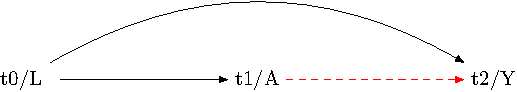
\includegraphics[width=0.8\textwidth,height=\textheight]{causal-dags_files/figure-pdf/fig-dag-common-cause-1.pdf}

}

\caption{\label{fig-dag-common-cause}Counfounding by a common cause. The
red path indicates bias arising from the open backdoor path from A to
Y.}

\end{figure}

\subsubsection{Advice: attend to the temporal order of all measured
variables}\label{advice-attend-to-the-temporal-order-of-all-measured-variables}

To address confounding by a common cause, one should adjust for it,
effectively blocking the backdoor path from the exposure to the outcome.
Essentially, conditioning on \(L\) separates \(A\) and \(Y\) in terms of
dependency. Standard methods for this adjustment include regression,
matching, inverse probability of treatment weighting, and G-methods, as
detailed in (\citeproc{ref-hernuxe1n2023}{Hernán and Monge 2023}).
Figure~\ref{fig-dag-common-cause-solution} highlights the necessity for
any confounder, as a common cause of both \(A\) and \(Y\), to precede
\(A\) chronologically, as causes precede their effects.

To manage the issue of confounding by a common cause, it is crucial to
maintain the correct temporal order:

\begin{enumerate}
\def\labelenumi{\arabic{enumi}.}
\tightlist
\item
  Measure all confounders \(L_{t0}\), which are common causes of both
  the exposure \(A_{t1}\) and the outcome \(Y_{t2}\).
\item
  Ensure that \(L_{t0}\) is measured before \(A_{t1}\) occurs.
\item
  Ensure that \(A_{t1}\) is measured before \(Y_{t2}\) occurs.
\end{enumerate}

After we have time-indexing the nodes on the graph it becomes evident
that \textbf{control of confounding generally requires time-series data
repeatedly measured on the units for which causal inferences apply.} Our
chronologically ordered causal diagram serves as a circuit breaker for
causal inferences in settings where researchers lack time series data.

\begin{figure}

{\centering 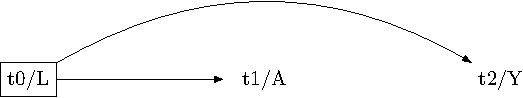
\includegraphics[width=0.8\textwidth,height=\textheight]{causal-dags_files/figure-pdf/fig-dag-common-cause-solution-1.pdf}

}

\caption{\label{fig-dag-common-cause-solution}Solution: adjust for
pre-exposure confounder. The implication: obtain time series data to
ensure the confounder occurs before the exposure.}

\end{figure}

\subsubsection{2. Confounding by conditioning on a common effect
(Collider
Stratification)}\label{confounding-by-conditioning-on-a-common-effect-collider-stratification}

When conditioning on a common effect, we consider a scenario where a
variable \(L\) is influenced by both a treatment \(A\) and an outcome
\(Y\) (\citeproc{ref-cole2010}{Cole \emph{et al.} 2010}).

Imagine \(A\) represents the level of belief in Big Gods, and \(Y\)
denotes social complexity, with \(L\) being economic trade. Initially,
suppose there is no causal link between \(A\) and \(Y\) --- altering
belief in Big Gods does not impact social complexity directly. However,
assume both \(A\) and \(Y\) independently affect economic trade (\(L\)).
If we analyze the data, ignoring the temporal sequence, particularly
when time series data are not available, or are measured with error, we
might mistakenly infer a causal relationship between \(A\) and \(Y\)
arising from their shared effect on \(L\).

In mathematical terms, when \(A\) and \(Y\) are independent, their joint
probability should equal the product of their individual probabilities:
\(P(A, Y) = P(A)P(Y)\). But, conditioning on \(L\) alters this
relationship. The joint probability of \(A\) and \(Y\) given \(L\),
\(P(A, Y | L)\), does not equal the product of \(P(A | L)\) and
\(P(Y | L)\). Thus, the common effect \(L\) creates an apparent
association between \(A\) and \(Y\), which is not causal. This spurious
association might lead to the false conclusion of a direct link between
beliefs in Big Gods and social complexity in cross-sectional data.

\begin{figure}

{\centering 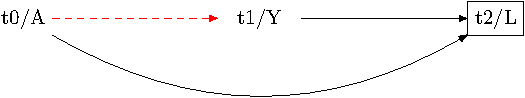
\includegraphics[width=0.8\textwidth,height=\textheight]{causal-dags_files/figure-pdf/fig-dag-common-effect-1.pdf}

}

\caption{\label{fig-dag-common-effect}Confounding by conditioning on a
collider. The dashed red path indicates bias from the open backdoor path
from A to Y.}

\end{figure}

\subsubsection{Advice: again, attend to the temporal order of all
measured
variables}\label{advice-again-attend-to-the-temporal-order-of-all-measured-variables}

To manage the issue of conditioning on a common effect, it is again
crucial to maintain the correct temporal order:

\begin{enumerate}
\def\labelenumi{\arabic{enumi}.}
\tightlist
\item
  Measure all confounders \(L_{t0}\), which are common causes of both
  the exposure \(A_{t1}\) and the outcome \(Y_{t2}\).
\item
  Ensure that \(L_{t0}\) is measured before \(A_{t1}\) occurs.
\item
  Ensure that \(A_{t1}\) is measured before \(Y_{t2}\) occurs.
\end{enumerate}

Adhering to this temporal sequence precludes \(L\) from being an effect
of either \(A\) or \(Y\).\footnote{7} In our example of beliefs and
social complexity, this typically necessitates time-series data with
precise measurements. Additionally, a sufficiently large sample of
cultures undergoing transitions in religious beliefs, with pre- and
post-transition measurements of social complexity, is needed. The
cultures in the dataset should also be independent of each other. That
is, each element of our causal inferential workflow must
cohere.\footnote{The independence of cultural units was at the centre of
  the study of comparative urban archaeology from the late 19th
  (\citeproc{ref-decoulanges1903}{De Coulanges 1903}) through the late
  20th century (\citeproc{ref-wheatley1971}{Wheatley 1971}). Despite
  attention to this problem in recent work (e.g.
  (\citeproc{ref-watts2016}{Watts \emph{et al.} 2016})), there is
  arguably a greater head-room for understanding the need for
  conditional independence of cultures in recent cultural evolutionary
  studies. Again, attending to the temporal order of events is
  essential.}

\begin{figure}

{\centering 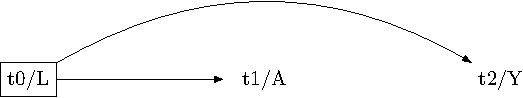
\includegraphics[width=0.8\textwidth,height=\textheight]{causal-dags_files/figure-pdf/fig-dag-common-effect-solution-1.pdf}

}

\caption{\label{fig-dag-common-effect-solution}Solution: time idexing of
confounders helps to avoid collider bias and maintain d-separation. The
graph makes the imperative clear: we must collect time series data with
confounders measured before the exposure, and that we must likewise
measure the exposure before the outcome, with data collected
repeatitively on the same units.}

\end{figure}

\subsubsection{3. Mediator Bias}\label{mediator-bias}

Mediator bias occurs when conditioning on a mediator, a variable that is
part of the causal pathway between the treatment and the outcome,
distorts the total effect of the treatment on the outcome.

Consider ``beliefs in Big Gods'' as the treatment \(A_{t0}\), ``social
complexity'' as the outcome \(Y_{t2}\), and ``economic trade'' as the
mediator \(L_{t1}\).

In this example, beliefs in Big Gods \(A_{t0}\) directly influence
economic trade \(L_{t1}\), which then affects social complexity
\(Y_{t2}\). Conditioning on economic trade \(L_{t1}\) can lead to biased
estimates of the overall effect of beliefs in Big Gods \(A\) on social
complexity \(Y_{t2}\). This bias arises because conditioning on \(L\)
might minimize the direct effect of \(A_{t0}\) on \(Y_{t1}\), blocking
the pathway through \(L_{t1}\). This is known as mediator bias,
illustrated in Figure~\ref{fig-dag-mediator}.

It might seem that conditioning on a mediator under a null hypothesis
(where \(A\) does not cause \(Y\)) would not introduce bias. However,
consider a situation where \(L_{t1}\) is affected by both the exposure
\(A_{t0}\) and an unmeasured variable \(U\) that is related to the
outcome \(Y_{t2}\). In this case, including \(L_{t1}\) in the analysis
might exaggerate the association between \(A_{t0}\) and \(Y_{t2}\), even
if there is no actual association between them and \(U\) does not cause
\(A_{t0}\). This scenario is depicted in
Figure~\ref{fig-dag-descendent}.

Therefore, unless specifically conducting mediation analysis, it is
generally inadvisable to condition on a post-treatment variable like
\(L_{t1}\). Attending to the temporal order in data collection is
crucial. If we cannot ensure that \(L\) is measured before \(A\), and if
\(A\) can influence \(L\), including \(L\) in our model could lead to
mediator bias. This scenario is represented in
Figure~\ref{fig-dag-descendent}.

You ask: ``What if \(L\) is a confounder of \(A\) and \(Y\)?'' We have
already considered this problem, and its solution. The problem was
presented in Figure~\ref{fig-dag-common-cause}. Our chronlogically
ordered causal diagram Figure~\ref{fig-dag-common-cause-solution}
directs us to the solution: \emph{If} \(L\) is a common cause of \(A\)
and \(Y\) we must ensure that our measurement of \(L\) occurs before our
measurement of \(A\) and that our measurement of \(Y\) occurs after our
measurement of \(A\).

\subsubsection{Advice: again, attend to the temporal order of all
measured
variables}\label{advice-again-attend-to-the-temporal-order-of-all-measured-variables-1}

To manage the issue of conditioning on a mediator, it is, yet again,
crucial to maintain the correct temporal order:

\begin{enumerate}
\def\labelenumi{\arabic{enumi}.}
\tightlist
\item
  Measure all confounders \(L_{t0}\), which are common causes of both
  the exposure \(A_{t1}\) and the outcome \(Y_{t2}\).
\item
  Ensure that \(L_{t0}\) is measured before \(A_{t1}\) occurs.
\item
  Ensure that \(A_{t1}\) is measured before \(Y_{t2}\) occurs.
\end{enumerate}

For we will only control for confounding if we have obtained \(L_{t0}\),
\(A_{t1}\), and \(Y_{t2}\), in the correct temporal sequence, and not
otherwise. Our graph again reveals demands not merely on the analysis of
data, but also of its collection.

\begin{figure}

{\centering 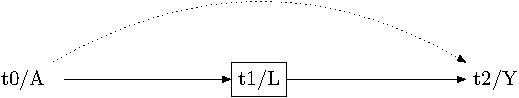
\includegraphics[width=0.8\textwidth,height=\textheight]{causal-dags_files/figure-pdf/fig-dag-mediator-1.pdf}

}

\caption{\label{fig-dag-mediator}Confounding by conditioning on a
mediator. The dashed black arrow indicates bias arising from partially
blocking the path between A and Y. Here, the true effect of A on Y is
attenuated.}

\end{figure}

\subsubsection{Advice: attend to the temporal order of all measured
variables}\label{advice-attend-to-the-temporal-order-of-all-measured-variables-1}

One should only condition on a mediator if our interest pre-specified
causal question requires a causal mediation model (The assumptions of
causal mediation are discussed in Section 3). Generally, we may avoid
mediation bias by ensuring that \(L\) is measured before the treatment
\(A\) and the outcome \(Y\). There are two exceptions to this rule. If
\(L\) were associated with \(Y\) and could not be caused by \(A\), then
conditioning on \(L\) would typically enhance the precision of the
causal effect estimate of \(A \to Y\). This precision enhancement holds
even if \(L\) occurs \emph{after} \(A\). A second a counter-example is
presented in Figure~\ref{fig-dag-descendent-solution-2} and developed in
the next section. However, when conditioning on a post-treatment
variable the onus is always on the researcher to explain why the
post-treatment variable cannot be affected by the exposure. Here again,
we discover the importance of explicitly stating the temporal ordering
of our variables in our graph.{[}\^{}10{]} Doing so directs us the data
we need to answer our causal question, and greatly diminishes the threat
of unwittingly introducing mediation bias.

\begin{figure}

{\centering 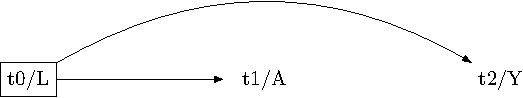
\includegraphics[width=0.8\textwidth,height=\textheight]{causal-dags_files/figure-pdf/fig-dag-mediator-solution-1.pdf}

}

\caption{\label{fig-dag-mediator-solution}Solution: do not condition on
a mediator. The implication: by ensuring temporal order in data
collection we diminish the probabilty of mistaking an effect of an
exposure for its confounder.}

\end{figure}

\subsubsection{4. Conditioning on a
descendant}\label{conditioning-on-a-descendant}

\paragraph{Case when conditioning on a descendant augments
bias}\label{case-when-conditioning-on-a-descendant-augments-bias}

Suppose a variable \(L\) is a cause of another variable \(L^\prime\).
Here, \(L^\prime\) is a descendant of \(L\). According to Markov
factorisation (see Appendix 2), if we were to condition on \(L\prime\),
we would also partially condition on \(L\).

Consider how conditioning on \(L\prime\) might imperil causal
estimation. Suppose there is a confounder \(L^\prime\) that is caused by
an unobserved variable \(U\), and is affected by the treatment \(A\).
Suppose further that \(U\) causes the outcome \(Y\). In this scenario,
as described in Figure~\ref{fig-dag-descendent}, conditioning on
\(L^\prime\), which is a descendant of \(A\) and \(U\), can lead to a
spurious association between \(A\) and \(Y\) through the path
\(A \to L^\prime \to U \to Y\).

\begin{figure}

{\centering 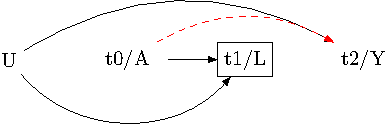
\includegraphics[width=0.8\textwidth,height=\textheight]{causal-dags_files/figure-pdf/fig-dag-descendent-1.pdf}

}

\caption{\label{fig-dag-descendent}Confounding by descent: the red path
illustrates the introduction of bias by conditioning on the descendant
of a confounder that is affected by the exposure, thus opening a path
between the exposure, A, and the outcome, Y.}

\end{figure}

\subsubsection{Solution to the problem of augmenting bias by
conditioning on a
descendant}\label{solution-to-the-problem-of-augmenting-bias-by-conditioning-on-a-descendant}

Again, the strategy for avoiding the problem of augmented bias by
conditioning on a descendant is evident from the chronology of the
graph. If we wish to reduce confounding we must ensure that \(L^\prime\)
is measured before the exposure \(A\). This strategy is presented in
Figure~\ref{fig-dag-descendent-solution}.

\begin{figure}

{\centering 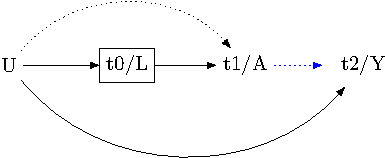
\includegraphics[width=0.8\textwidth,height=\textheight]{causal-dags_files/figure-pdf/fig-dag-descendent-solution-1.pdf}

}

\caption{\label{fig-dag-descendent-solution}Solution: measure L before
A. Note, L need not affect Y to be a confounder (i.e.~a member of a
confounder set).}

\end{figure}

\paragraph{Case when conditioning on a descendant reduces
bias}\label{case-when-conditioning-on-a-descendant-reduces-bias}

Next consider a case in which we may use a post-treatment descendent to
reduce bias. Suppose an unmeasured confounder \(U\) affects \(A\),
\(Y\), and \(L^\prime\) in an effect of \(U\) that occurs after \(A\)
and \(Y\). In this scenario adjusting for \(L^\prime\) may help to
reduce confounding caused by the unmeasured confounder \(U\). This
strategy follows from the modified disjunctive cause criterion for
confounding control, we recommends that we ``include as a covariate any
proxy for an unmeasured variable that is a common cause of both the
exposure and the outcome'' (\citeproc{ref-vanderweele2019}{VanderWeele
2019}). As shown in Figure~\ref{fig-dag-descendent-solution-2}, although
\(L^\prime\) occurs \emph{after} the exposure, and indeed occur
\emph{after} the outcome, coniditioning on it will reduce confounding.
How might this work? Consider a genetic factor that affects the exposure
and the outcome early in life but which is expressed later later in
life. Adjusting for such an expression of the genetic factor that
expresses later in life would help use to control for the unmeasured
confounding by common cause from the genetic factors influence on \(A\)
and \(Y\), which again are imagined to occur before \(L'\). Here
conditioning on \(L'\) is sensible, and provides an example of
post-outcome confounding control. This scenario is presented in
Figure~\ref{fig-dag-descendent-solution-2}.

\textbf{This scenario reveals that thoughlessly following a simple rule
that requires us to condition only on pre-exposure (and indeed
pre-outcome) variables would be hasty.} More generally, demonstrates the
imperative for thinking carefully about data collection. Each problem
must be approached anew. Here we find that causal diagrams are a great
benefit. For if we are able to provide a structural representation of
confounding, we merely need to inspect the graph to ensure that all
backdoor paths are closed.

\begin{figure}

{\centering 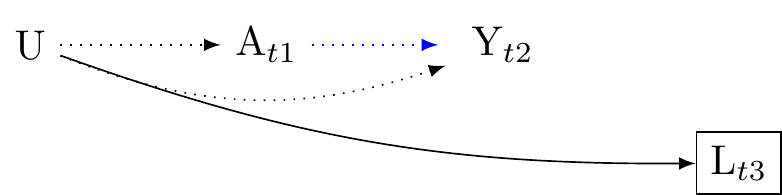
\includegraphics[width=0.8\textwidth,height=\textheight]{causal-dags_files/figure-pdf/fig-dag-descendent-solution-2-1.pdf}

}

\caption{\label{fig-dag-descendent-solution-2}Solution: conditioning on
a confounder that occurs after the exposure and the outcome might
address a problem of unmeasured confounding if the confounder is a
descendent of a prior common cause of the exposure and outcome. The
dotted paths denote that the effect of U on A and Y is partially blocked
by conditioning on L', even though L' occurs after the outcome. The
paths are dotted to represent a reduction of bias by conditioning on the
post-outcome descendent of an unmeasured common cause of the exposure
and outcome.}

\end{figure}

\subsubsection{M-bias: Conditioning on an Instrumental Variable Before
the Exposure May Introduce
Bias}\label{m-bias-conditioning-on-an-instrumental-variable-before-the-exposure-may-introduce-bias}

While it is generally advisable to include indicators for confounders
that are measured before their corresponding exposures, there are
caveats. One must be cautious not to over-condition on pre-exposure
variables that are not associated with both the exposure and confounder.
Such over-conditioning may inadvertently induce confounding, known as
``M-bias.''

As illustrated in Figure~\ref{fig-m-bias}, M-bias can occur even if a
variable \(L\) occurs before the treatment \(A\). This happens when
\(L\) does not affect either \(A\) or \(Y\), but is a descendant of
unmeasured variables that influence both \(A\) and \(Y\) independently.
Conditioning on \(L\) creates a spurious association between \(A\) and
\(Y\). In such cases, \(A\) and \(Y\) might be unconditionally
independent (\(A \coprod Y(a)\)), but when stratified by \(L\),
independence is violated: (\(A \cancel{\coprod} Y(a)| L\)). This form of
bias is another manifestation of collider stratification bias.

Note that when the path is ordered chronologically from left to right,
the ``M'' shape, giving M-bias its name, changes to an ``E'' shape.
However, the term ``M-bias'' is retained.

\subsubsection{Advice: Adopt the Modified Disjunctive Cause
Criterion}\label{advice-adopt-the-modified-disjunctive-cause-criterion}

The modified disjunctive cause criterion offers a strategy to satisfy
the backdoor criterion and reduce bias:

\begin{enumerate}
\def\labelenumi{\alph{enumi}.}
\tightlist
\item
  Control for any variable that causes the exposure, the outcome, or
  both.
\item
  Control for any proxy for an unmeasured variable that is a shared
  cause of both exposure and outcome.
\item
  Define an instrumental variable as one associated with the exposure
  but not independently influencing the outcome, except through the
  exposure. Exclude any instrumental variable that is not a proxy for an
  unmeasured confounder from the confounder set.
\end{enumerate}

Determining which variables belong in the confounder set can be
challenging. Specialist knowledge often plays a key role here, as the
data alone may not provide clear guidance. This approach is supported by
various sources, including VanderWeele \emph{et al.}
(\citeproc{ref-vanderweele2020}{2020}) and VanderWeele
(\citeproc{ref-vanderweele2019}{2019}), with specific exceptions noted
in sources like bulbulia2021.

Typically, indicators for confounders should be included only if they
are known to be measured before their exposures - with notable
exceptions described below in fig-dag-descendent-solution-2 and .

However, researchers should also be cautious about over-conditioning on
pre-exposure variables that are not associated with both the exposure
and confounder, as doing so can induce confounding. As shown in
Figure~\ref{fig-m-bias}, collider stratification may arise even if \(L\)
occurs before \(A\). This happens when \(L\) does not affect \(A\) or
\(Y\), but may be the descendent of an unmeasured variable that affects
\(A\) and another unmeasured variable that also affects \(Y\).
Conditioning on \(L\) in this scenario evokes ``M-bias.'' If \(L\) is
not a common cause of \(A\) and \(Y\), or the effect of a shared common
cause, \(L\) should not be included in a causal model.
Figure~\ref{fig-m-bias} presents a case in which \(A \coprod Y(a)\) but
\(A \cancel{\coprod} Y(a)| L\). M-bias is another example of collider
stratification bias (see: (\citeproc{ref-cole2010}{Cole \emph{et al.}
2010})).\footnote{Note, when we draw a chronologically ordered path from
  left to right the M shape for which ``M-bias'' takes its name changes
  to an E shape We shall avoid proliferating jargon and retain the term
  ``M bias.''}

\begin{figure}

{\centering 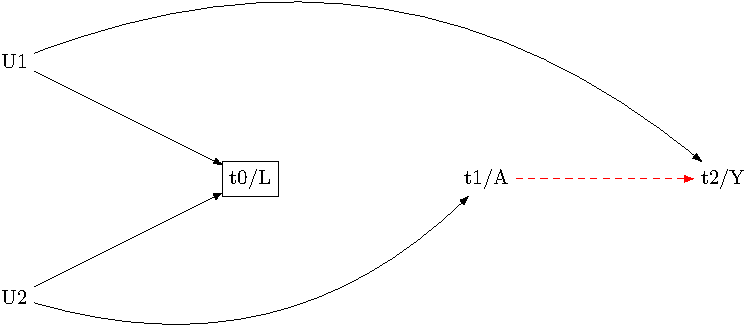
\includegraphics[width=0.8\textwidth,height=\textheight]{causal-dags_files/figure-pdf/fig-m-bias-1.pdf}

}

\caption{\label{fig-m-bias}M-bias: Confounding control by including
previous outcome measures. The dashed red path indicates bias from the
open backdoor path from A to Y by conditioning on pre-exposure variable
L. The solution: do not condition on L. The graph shows that
conditioning on variables measured before the exposure is not sufficient
to prevent confounding.}

\end{figure}

\subsubsection{Advice: Adopt the Modified Disjunctive Cause Criterion
for Confounding
Control}\label{advice-adopt-the-modified-disjunctive-cause-criterion-for-confounding-control}

The modified disjunctive cause criterion offers a strategy to satisfy
the backdoor criterion and reduce bias:

\begin{enumerate}
\def\labelenumi{\alph{enumi}.}
\tightlist
\item
  Control for any variable that causes the exposure, the outcome, or
  both.
\item
  Control for any proxy for an unmeasured variable that is a shared
  cause of both exposure and outcome.
\item
  Define an instrumental variable as one associated with the exposure
  but not independently influencing the outcome, except through the
  exposure. Exclude any instrumental variable that is not a proxy for an
  unmeasured confounder from the confounder set.
\end{enumerate}

Determining which variables belong in the confounder set can be
challenging. Specialist knowledge often plays a key role here, as the
data alone may not provide clear guidance. For more discussion of the
modified disjunctive cause criterion see: VanderWeele \emph{et al.}
(\citeproc{ref-vanderweele2020}{2020}) and VanderWeele
(\citeproc{ref-vanderweele2019}{2019}).

\subsection{Part 3. Application of Causal Diagrams for Clarifying
Moderation (Interaction), Mediation, and Longitudinal
Feedback}\label{part-3.-application-of-causal-diagrams-for-clarifying-moderation-interaction-mediation-and-longitudinal-feedback}

\subsubsection{Case 1. Causal Interaction and Causal Effect
Modification: do not draw non-linear relationships such as
interactions}\label{case-1.-causal-interaction-and-causal-effect-modification-do-not-draw-non-linear-relationships-such-as-interactions}

Interactions are scientific interesting because we often wish to
understand whether causal effects operate differently in different
sub-populations, or whether the joint effect of two interventions differ
from the either taken alone, and from no intervention.

How shall we depict interactions on a graph? It is crucial to remember
the primary function of causal diagrams is to investigate confounding.
Causal diagrams are not designed to capture all facets of a phenomenon
under investigation. We should not attempt any unique visual trick to
show additive and multiplicative interaction by, for example, presenting
arrows intersecting arrows. Moreover, we should include those nodes and
paths that are necessary to evaluate structural sources of bias. Causal
graphs are meant to be human readable. They are not meant to be complete
maps of causal reality.

In my experience, misunderstandings arise about the role and function of
causal diagrams in application to interaction are not simply confusions
about graphical convention. Misunderstanding typically stems from a more
profound confusion about the concept of interaction itself.

Given this deeper problem, it is worth clarifying two distinct
conceptions of causal interaction as understood within the
counterfactual causal framework: the concept of causal interaction as a
double exposure and the concept of causal effect-modification from a
single exposure.

\paragraph{\texorpdfstring{\textbf{Causal interaction as a double
exposure}}{Causal interaction as a double exposure}}\label{causal-interaction-as-a-double-exposure}

Causal interaction refers to the combined and separate effect of two
exposures. Evidence for interaction on a given scale is present when the
effect of one exposure on an outcome depends on another exposure's
level. For instance, the impact of beliefs in Big Gods (exposure \(A\))
on social complexity (outcome \(Y\)) might depend on a culture's
monumental architecture (exposure \(B\)), which could also influence
social complexity. Evidence of causal interaction on the difference
scale would be present if:

\[\bigg(\underbrace{\mathbb{E}[Y(1,1)]}_{\text{joint exposure}} - \underbrace{\mathbb{E}[Y(0,0)]}_{\text{neither exposed}}\bigg) - \bigg[ \bigg(\underbrace{\mathbb{E}[Y(1,0)]}_{\text{only A exposed}} - \underbrace{\mathbb{E}[Y(0,0)]}_{\text{neither exposed}}\bigg) + \bigg(\underbrace{\mathbb{E}[Y(0,1)]}_{\text{only B exposed}} - \underbrace{\mathbb{E}[Y(0,0)]}_{\text{neither exposed}} \bigg)\bigg] \neq 0 \]

This equation simplifies to

\[ \underbrace{\mathbb{E}[Y(1,1)]}_{\text{joint exposure}} - \underbrace{\mathbb{E}[Y(1,0)]}_{\text{only A exposed}} - \underbrace{\mathbb{E}[Y(0,1)]}_{\text{only B exposed}} + \underbrace{\mathbb{E}[Y(0,0)]}_{\text{neither exposed}} \neq 0 \]

If the above equation were to hold, the effect of exposure \(A\) on the
outcome \(Y\) would differ across levels of \(B\) or vice versa. Such a
difference would provide evidence for interaction.

If the value is positive, we say there is evidence for an additive
effect. If the value is less than zero, we say there is evidence for a
sub-additive effect. If the value is virtually zero, there is no
reliable evidence for interaction.\footnote{Note that causal effects of
  interactions often differ when measured on the ratio scale. This
  discrepency can have significant policy implications, see:
  (\citeproc{ref-vanderweele2014}{VanderWeele and Knol 2014}). Although
  beyond the scope of this article, when evaluating evidence for
  causality we must clarify the measure of effect in which we are
  interested (\citeproc{ref-hernuxe1n2004}{Hernán 2004};
  \citeproc{ref-tripepi2007}{Tripepi \emph{et al.} 2007}).}

Remember that causal diagrams are non-parametric. They do not directly
represent interactions. They are tools for addressing the identification
problem. Although a causal diagram can indicate an interaction's
presence by displaying two exposures jointly influencing an outcome, as
in Figure~\ref{fig-dag-interaction}, it does not directly represent the
interaction's nature or scale.

\begin{figure}

{\centering 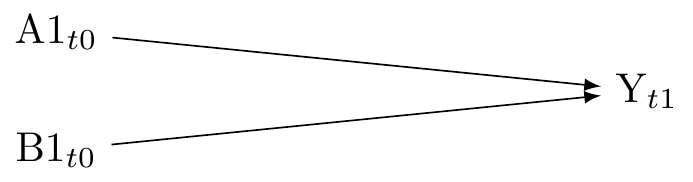
\includegraphics[width=0.6\textwidth,height=\textheight]{causal-dags_files/figure-pdf/fig-dag-interaction-1.pdf}

}

\caption{\label{fig-dag-interaction}Causal interaction: if two exposures
are causally independent of each other, we may wish to estimate their
individual and joint effects on Y, conditional on confounding control
strategy that blocks backdoor paths for bothe exposures (here, L1 and L2
are jointly required). where the counterfactual outcome is Y(a,b) and
there is evidence for additive or subadditive interaction if E{[}Y(1,1)
- Y(0,1) - Y(1,0) + Y(0,0){]} ≠ 0. If we cannot conceptualise B as a
variable upon which intervention can occur, then the interaction is
better conceived as effect modification (see next figure). Important: do
not attempt to draw a path into another path.}

\end{figure}

\paragraph{\texorpdfstring{\textbf{Causal effect modification under a
single
exposure}}{Causal effect modification under a single exposure}}\label{causal-effect-modification-under-a-single-exposure}

With the analysis of effect modification, we aim to understand how an
exposure's effect varies, if at all, across levels of another variable,
an effect modifier.

Consider again the problem of estimating the causal effect of beliefs in
Big Gods on social complexity. Suppose this time we are interested in
the investigating whether this effect varies across early urban
civilisations in ancient China and South America. In this example
geography (China versus South America) is an ``effect modifier.'' Here,
we do not treat the effect modifier as an intervention. Rather, we wish
to investigate whether geography is a parameter that may alter the
exposure's effect on an outcome.

FFor clarity, let's consider two exposure levels, denoted as \(A = a\)
and \(A = a^*\). Additionally, assume that \(G\) represents two distinct
groups, such as \(g\) and \(g'\), where these groups could be based on
different geographical characteristics.

The expected outcome when the exposure is at level \(A = a\) among
individuals in group \(G = g\) is expressed as:

\[\hat{E}[Y(a)|G=g]\]

This represents the average outcome under exposure \(a\) for group
\(g\).

Similarly, the expected outcome for exposure level \(A = a^*\) among
individuals in the same group (\(G = g\)) is:

\[\hat{E}[Y(a^*)|G=g]\]

The causal effect of shifting the exposure level from \(a^*\) to \(a\)
within group \(g\) is then given by:

\[\hat{\delta}_g = \hat{E}[Y(a)|G=g] - \hat{E}[Y(a^*)|G=g]\]

This measures the change in the expected outcome due to altering the
exposure from \(a^*\) to \(a\) within group \(g\).

Likewise, the causal effect of changing the exposure from \(a^*\) to
\(a\) within group \(g'\) is expressed as:

\[\hat{\delta}_{g'} = \hat{E}[Y(a)|G=g'] - \hat{E}[Y(a^*)|G=g']\]

Here, \(\hat{\delta}_{g'}\) captures the analogous effect in group
\(g'\).

To compare the causal effect on a difference scale between these two
groups, we calculate:

\[\hat{\gamma} = \hat{\delta}_g - \hat{\delta}_{g'}\]

The value of \(\hat{\gamma}\) quantifies the differential effect of
shifting the exposure from \(a^*\) to \(a\) between groups \(g\) and
\(g'\). A non-zero \(\hat{\gamma}\) indicates evidence of effect
modification, suggesting that the impact of changing the exposure varies
based on group characteristics. If \(G\) represents a geographic
distinction, then \(\hat{\gamma} \neq 0\) would suggest geographical
variation in the exposure effect. However, if \(G\) denotes other types
of groups, \(\hat{\gamma}\) reflects effect modification according to
those specific group characteristics, in this example, geographical
characteristics.

Again, remember that causal diagrams are non-parametric. More
fundamental, causal diagrams function to identify structural sources of
bias and to help researchers develop strategies for addressing such
bias. We should not draw an intersecting path or attempt other
visualisations to represent effect modification. Instead, we should draw
two edges into the exposure. This is depicted in
Figure~\ref{fig-dag-effect-modfication}.\footnote{For distinctions
  within varieties of effect modification relevant for strategies of
  confounding controul see (\citeproc{ref-vanderweele2007}{VanderWeele
  and Robins 2007}).}

\begin{figure}

{\centering 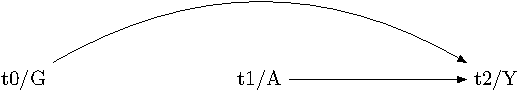
\includegraphics[width=0.8\textwidth,height=\textheight]{causal-dags_files/figure-pdf/fig-dag-effect-modfication-1.pdf}

}

\caption{\label{fig-dag-effect-modfication}A simple graph for
effect-modification in which there are no confounders. G is an effect
modifier of A on Y. We draw a box around G to indicate we are
conditioning on this variable.}

\end{figure}

\subsubsection{Case 2: Causal mediation: causal diagrams reveal the
inadequacy of standard
approaches}\label{case-2-causal-mediation-causal-diagrams-reveal-the-inadequacy-of-standard-approaches}

The conditions necessary for causal mediation are stringent. I present
these conditions in the chronologically ordered causal diagram shown in
Figure~\ref{fig-dag-mediation-assumptions}. We will again consider
whether cultural beliefs in Big Gods affect social complexity. We now
ask whether this affect is mediated by political authority. The
assumptions required for asking causal mediation questions are as
follows

\begin{enumerate}
\def\labelenumi{\arabic{enumi}.}
\tightlist
\item
  \textbf{No unmeasured exposure-outcome confounder}
\end{enumerate}

This prerequisite is expressed: \(Y(a,m) \coprod A | L1\). Upon
controlling for the covariate set \(L1\), we must ensure that no
additional unmeasured confounders affect both the cultural beliefs in
Big Gods \(A\) and the social complexity \(Y\). For example, suppose our
study involves the effect of cultural beliefs in Big Gods (exposure) on
social complexity (outcome), and geographic location and historical
context define the covariates in \(L1\). In that case, we must assume
that accounting for \(L1\) d-separates \(A\) and \(Y\). The relevant
confounding path is depicted in brown in
Figure~\ref{fig-dag-mediation-assumptions}.

\begin{enumerate}
\def\labelenumi{\arabic{enumi}.}
\setcounter{enumi}{1}
\tightlist
\item
  \textbf{No unmeasured mediator-outcome confounder}
\end{enumerate}

This condition is expressed: \(Y(a,m) \coprod M | L2\). After
controlling for the covariate set \(L2\), we must ensure that no other
unmeasured confounders affect the political authority \(M\) and social
complexity \(Y\). For instance, if trade networks impact political
authority and social complexity, we must account for trade networks to
obstruct the unblocked path linking our mediator and outcome. Further,
we must assume the absence of any other confounders for the
mediator-outcome path. This confounding path is represented in blue in
Figure~\ref{fig-dag-mediation-assumptions}.

\begin{enumerate}
\def\labelenumi{\arabic{enumi}.}
\setcounter{enumi}{2}
\tightlist
\item
  \textbf{No unmeasured exposure-mediator confounder}
\end{enumerate}

This requirement is expressed: \(M(a) \coprod A | L3\). Upon controlling
for the covariate set \(L3\), we must ensure that no additional
unmeasured confounders affect both the cultural beliefs in Big Gods
\(A\) and political authority \(M\). For example, the capability to
construct large ritual theatres may influence the belief in Big Gods and
the level of political authority. If we have indicators for this
technology measured prior to the emergence of Big Gods (these indicators
being \(L3\)), we must assume that accounting for \(L3\) closes the
backdoor path between the exposure and the mediator. This confounding
path is shown in green in Figure~\ref{fig-dag-mediation-assumptions}.

\begin{enumerate}
\def\labelenumi{\arabic{enumi}.}
\setcounter{enumi}{3}
\tightlist
\item
  \textbf{No mediator-outcome confounder affected by the exposure}
\end{enumerate}

This requirement is expressed: \(Y(a,m) \coprod M(a^*) | L\). We must
ensure that no variables confounding the relationship between political
authority and social complexity in \(L2\) are themselves influenced by
the cultural beliefs in Big Gods (\(A\)). For instance, when studying
the effect of cultural beliefs in Big Gods (\(A\), the exposure) on
social complexity (\(Y\), the outcome) as mediated by political
authority (mediator), there can be no factors, such as trade networks
(\(L2\)), that influence both political authority and social complexity
and are affected by the belief in Big Gods. This confounding path is
shown in red in Figure~\ref{fig-dag-mediation-assumptions}. \textbf{Note
that the assumption of no exposure-induced confounding in the
mediator-outcome relationship is often a substantial obstacle for causal
mediation analysis.} If the exposure influences a confounder of the
mediator and outcome, we face a dilemma. Without accounting for this
confounder, the backdoor path between the mediator and the outcome
remains open. By accounting for it, however, we partially obstruct the
path between the exposure and the mediator, leading to bias.
Consequently, observed data cannot identify the natural direct and
indirect effects.

Notice again that the requirements for counterfactual data science are
more strict than for descriptive or predictive data science.

We have now considered how chronologically ordered causal diagrams
elucidate the conditions necessary for causal mediation
analysis.\footnote{An excellent resource both for understanding causal
  interaction and causal mediation is
  (\citeproc{ref-vanderweele2015}{VanderWeele 2015}).}

\begin{figure}

{\centering \includegraphics[width=1\textwidth,height=\textheight]{causal-dags_files/figure-pdf/fig-dag-mediation-assumptions-1.pdf}

}

\caption{\label{fig-dag-mediation-assumptions}This causal diagram
illustrates the four fundamental assumptions needed for causal mediation
analysis. The first assumption pertains to the brown paths. It requires
the absence of an unmeasured exposure-outcome confounder, and assumes
that conditioning on L1 is sufficient for such confounding control. The
second assumption pertains to the blue paths. It requires the absence of
an unmeasured mediator-outcome confounder, and assumes that conditioning
on L2 is sufficient for such confounding control. The third assumption
pertains to the green paths. It requires the absence of an unmeasured
exposure-mediator confounder, and assumes that conditioning on L3 is
sufficient for such confounding control. The fourth and final assumption
pertains to the red paths. It requires the absence of an a
mediator-outcome confounder that is affected by the exposure, and
assumes that there is no path from the exposure to L2 to M. If the
exposure were to affect L2, then conditioning on L2 would block the
exposure's effect on the mediator, as indicated by dashed red path.
Causal diagrams not only clarify how different types of confounding bias
may converge (here mediation bias and confounder bias), but also reveal
the limitations of common methods such as structural equation models and
multilevel models for handling time-series data where the fourth
assumption fails -- that is, where there is treatment-confounder
feedback. Such feedback is common in time-series data, but not widely
understood. For example structural equation models and multi-level
models cannot address causal questions in the presence of such feedback,
but these models remain widely favoured.}

\end{figure}

\subsubsection{Case 3: Confounder-treatment feedback: longitudinal
``growth'' is not
causation}\label{case-3-confounder-treatment-feedback-longitudinal-growth-is-not-causation}

In our discussion of causal mediation, we consider how the effects of
two sequential exposures may combine to affect an outcome. We can
broaden this interest to consider the causal effects of multiple
sequential exposures. In such scenarios, causal diagrams arranged
chronologically can aid in clarifying the challenges and opportunities.

For example, consider temporally fixed multiple exposures. The
counterfactual outcomes may be denoted \(Y(a_{t1} ,a_{t2})\). There are
four counterfactual outcomes corresponding to the four fixed ``treatment
regimes:''

\begin{enumerate}
\def\labelenumi{\arabic{enumi}.}
\item
  \textbf{Always treat (Y(1,1))}
\item
  \textbf{Never treat (Y(0,0))}
\item
  \textbf{Treat once first (Y(1,0))}
\item
  \textbf{Treat once second (Y(0,1))}
\end{enumerate}

\phantomsection\label{tbl-regimes}
\begin{longtable}[]{@{}
  >{\raggedright\arraybackslash}p{(\columnwidth - 4\tabcolsep) * \real{0.1351}}
  >{\raggedright\arraybackslash}p{(\columnwidth - 4\tabcolsep) * \real{0.5405}}
  >{\raggedright\arraybackslash}p{(\columnwidth - 4\tabcolsep) * \real{0.3243}}@{}}
\caption{\label{tbl-regimes}Table describes four fixed treatment regimes
and six causal contrasts in time series data where the exposure may
vary.}\tabularnewline
\toprule\noalign{}
\begin{minipage}[b]{\linewidth}\raggedright
Type
\end{minipage} & \begin{minipage}[b]{\linewidth}\raggedright
Description
\end{minipage} & \begin{minipage}[b]{\linewidth}\raggedright
Counterfactual Outcome
\end{minipage} \\
\midrule\noalign{}
\endfirsthead
\toprule\noalign{}
\begin{minipage}[b]{\linewidth}\raggedright
Type
\end{minipage} & \begin{minipage}[b]{\linewidth}\raggedright
Description
\end{minipage} & \begin{minipage}[b]{\linewidth}\raggedright
Counterfactual Outcome
\end{minipage} \\
\midrule\noalign{}
\endhead
\bottomrule\noalign{}
\endlastfoot
Regime & Always treat & Y(1,1) \\
Regime & Never treat & Y(0,0) \\
Regime & Treat once first & Y(1,0) \\
Regime & Treat once second & Y(0,1) \\
Contrast & Always treat vs.~Never treat & E{[}Y(1,1) - Y(0,0){]} \\
Contrast & Always treat vs.~Treat once first & E{[}Y(1,1) - Y(1,0){]} \\
Contrast & Always treat vs.~Treat once second & E{[}Y(1,1) -
Y(0,1){]} \\
Contrast & Never treat vs.~Treat once first & E{[}Y(0,0) - Y(1,0){]} \\
Contrast & Never treat vs.~Treat once second & E{[}Y(0,0) - Y(0,1){]} \\
Contrast & Treat once first vs.~Treat once second & E{[}Y(1,0) -
Y(0,1){]} \\
\end{longtable}

There are six causal contrasts that we might compute for the four fixed
regimes, presented in Table~\ref{tbl-regimes}.\footnote{We compute the
  number of possible combinations of contrasts by
  \(C(n, r) = \frac{n!}{(n-r)! \cdot r!}\)}

Not that treatment assignments might be sensibly approached as a
function of the previous outcome. For example, we might \textbf{treat
once first} and then decide whether to treat again depending on the
outcome of the initial treatment. This aspect is known as ``time-varying
treatment regimes.''

Bear in mind that to estimate the ``effect'' of a time-varying treatment
regime, we are obligated to make comparisons between the relevant
counterfactual quantities. As mediation can introduce the possibility of
time-varying confounding (condition 4: the exposure must not impact the
confounders of the mediator/outcome path), the same holds true for all
sequential time-varying treatments. However, unlike conventional causal
mediation analysis, it might be necessary to consider the sequence of
treatment regimes over an indefinitely long period.

Chronologically organised causal diagrams are useful for highlighting
problems with traditional multi-level regression analysis and structural
equation modelling.

For example, we might be interested in whether belief in Big Gods
affects social complexity. Consider estimating a fixed treatment regime
first. Suppose we have a well-defined concept of Big Gods and social
complexity as well as excellent measurements for both over time. In that
case, we might want to assess the effects of beliefs in Big Gods on
social complexity, say, two centuries after the beliefs were introduced.

The fixed treatment strategies are: ``always believe in Big Gods''
versus ``never believe in Big Gods'' on the level of social complexity.
Refer to Figure~\ref{fig-dag-9}. Here, \(A_{tx}\) represents the
cultural belief in Big Gods at time \(tx\), and \(Y_{tx}\) is the
outcome, social complexity, at time \(x\). Imagine that economic trade,
denoted as \(L_{tx}\), is a time-varying confounder. Suppose its effect
changes over time, which in turns affects the factors that influence
economic trade. To complete our causal diagram, we might include an
unmeasured confounder \(U\), such as oral traditions, which could
influence both the belief in Big Gods and social complexity.

Consider a scenario where we can reasonably infer that the level of
economic trade at time \(0\), represented as \(L_{t0}\), impacts beliefs
in ``Big Gods'' at time \(1\), denoted as \(A_{t1}\). In this case, we
would draw an arrow from \(L_{t0}\) to \(A_{t1}\). Conversely, if we
assume that belief in ``Big Gods,'' \(A_{t1}\), influences the future
level of economic trade, \(L_{t2}\), then an arrow should be added from
\(A_{t1}\) to \(L_{t2}\). This causal diagram illustrates a feedback
process between the time-varying exposure \(A\) and the time-varying
confounder \(L\). Figure~\ref{fig-dag-9}. displays exposure-confounder
feedback. In practical settings, the diagram could contain more arrows.
However, the intention here is to use the minimal number of arrows
needed to demonstrate the issue of exposure-confounder feedback. As a
guideline, we should avoid overcomplicating our causal diagrams and aim
to include only the essential details necessary for assessing the
identification problem.

What would happen if we were to condition on the time-varying confounder
\(L_{t3}\)? Two things would occur. First, we would block all the
backdoor paths between the exposure \(A_{t2}\) and the outcome. We need
to block those paths to eliminate confounding. Therefore, conditioning
on the time-varying confounding is essential. However, paths that were
previously blocked would close. For example, the path
\(A_{t1}, L_{t2}, U, Y_{t4}\), that was previously closed would be
opened because the time-varying confounder is the common effect of
\(A_{t1}\) and \(U\). Conditioning, then, opens the path
\(A_{t1}, L_{t2}, U, Y_{t4}\). Therefore we must avoid conditioning on
the time-varying confounder. It would seem then that if we were to
condition on a confounder that is affected by the prior exposure, we are
``damned if we do'' and ``dammed if we do not.''

\begin{figure}

{\centering 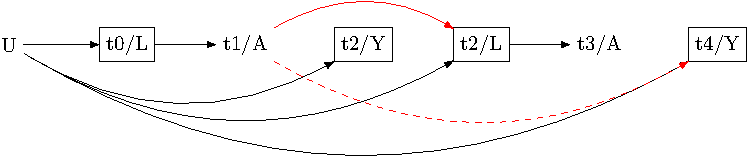
\includegraphics[width=1\textwidth,height=\textheight]{causal-dags_files/figure-pdf/fig-dag-9-1.pdf}

}

\caption{\label{fig-dag-9}Exposure confounder feedback is a problem for
time-series models. If we do not condition on L\_t2, a backdoor path is
open from A\_t3 to Y\_t4. However, if conditioning on L\_t2 introduces
collider bias, opening a path, coloured in red, between A\_t2 and Y\_t4.
Here, we may not use conventional methods to estimate the effects of
multiple exposures. Instead, at best, we may obtain controlled effects
using G-methods. Multi-level models will not eliminate bias (!).
However, outside of epidemiology, G-methods are presently rarely used.}

\end{figure}

A similar problem arises when a time-varying exposure and time-varying
confounder share a common cause. This problem arises even without the
exposure affecting the confounder. The problem is presented in
Figure~\ref{fig-dag-time-vary-common-cause-A1-l1}.

\begin{figure}

{\centering 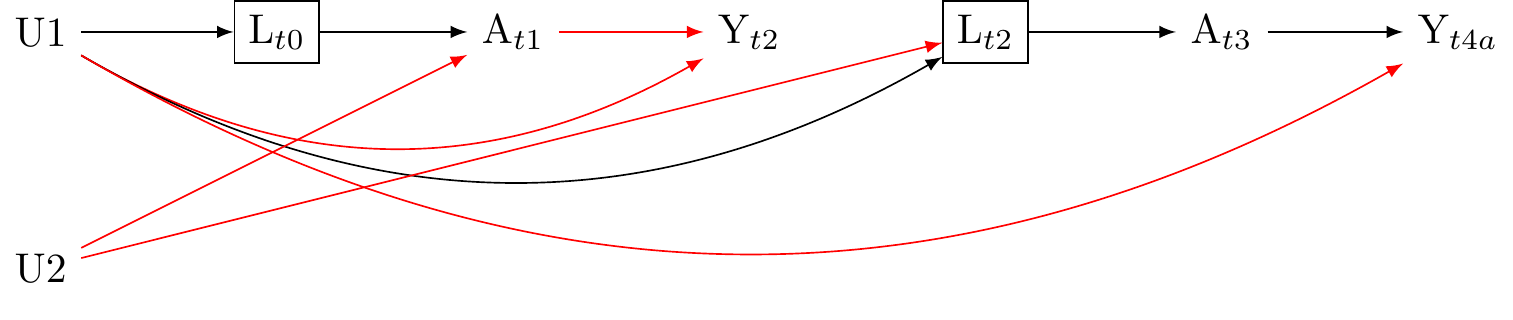
\includegraphics[width=1\textwidth,height=\textheight]{causal-dags_files/figure-pdf/fig-dag-time-vary-common-cause-A1-l1-1.pdf}

}

\caption{\label{fig-dag-time-vary-common-cause-A1-l1}Exposure confounder
feedback is a problem for time-series models. Here, the problem arises
from an unmeasured variable (U\_2) that affects both the exposure A at
time 1 and the cofounder L at time 2. The red paths show the open
backdoor path when we condition on the L at time 2. Again, we cannot
infer causal effects in such scenarios by using regression-based
methods. In this setting, to address causal questions, we require
G-methods.}

\end{figure}

The potential for confounding increases when the exposure \(A_{t1}\)
affects the outcome \(Y_{t4}\). For example, since \(L_{t2}\) is on the
path from \(A_{t1}\) to \(Y_{t4}\), conditioning on \(L_{t2}\) partially
blocks the relation between the exposure and the outcome, triggering
collider stratification bias and mediator bias. However, to close the
open backdoor path from \(L_{t2}\) to \(Y_{t4}\), it becomes necessary
to condition on \(L_{t2}\). Paradoxically, we have just stated that
conditioning should be avoided! This broader dilemma of
exposure-confounder feedback is thoroughly explored in
(\citeproc{ref-hernuxe1n2023}{Hernán and Monge 2023}). Treatment
confounder feedback is particularly challenging for evolutionary human
science, yet its handling is beyond the capabilities of conventional
regression-based methods, including multi-level models
(\citeproc{ref-hernuxe1n2006}{Hernán and Robins 2006};
\citeproc{ref-robins1986}{Robins 1986}; \citeproc{ref-robins1999}{Robins
\emph{et al.} 1999}). As mentioned previously, G-methods encompass
models appropriate for investigating the causal effects of both
time-fixed and time-varying exposures
(\citeproc{ref-chatton2020}{Chatton \emph{et al.} 2020};
\citeproc{ref-hernuxe1n2006}{Hernán and Robins 2006};
\citeproc{ref-naimi2017}{Naimi \emph{et al.} 2017}). Despite significant
recent advancements in the health sciences
(\citeproc{ref-breskin2021}{Breskin \emph{et al.} 2021};
\citeproc{ref-duxedaz2021}{Díaz \emph{et al.} 2021};
\citeproc{ref-williams2021}{Williams and Díaz 2021}), these methods have
not been widely embraced in the field of human evolutionary sciences
\footnote{It is worth noting that the identification of controlled
  effect estimates can be enhanced by graphical methods such as ``Single
  World Intervention Graphs'' (SWIGs), which represent counterfactual
  outcomes in the diagrams. However, SWIGs are more accurately
  considered templates rather than causal diagrams in their general
  form. The use of SWIGs extends beyond the scope of this tutorial. For
  more information, see Richardson and Robins
  (\citeproc{ref-richardson2013}{2013}).}

\subsubsection{Summary}\label{summary}

To consistently estimate causal effects, we must contrast the world as
it has been with the world as it might have been. For many questions in
evolutionary human science, we have seen that confounder-treatment
feedback leads to intractable causal identification problems. We have
also seen that causal diagrams are helpful in clarifying these problems.
Many self-inflicted injuries, such as mediator bias and
post-stratification bias, could be avoided if confounders were measured
prior to the exposures. Chronologically ordered causal diagrams aim to
make this basis transparent. They function as circuit-breakers that may
protect us from blowing up our causal inferences. More constructively,
temporal order in the graph focusses attention on imperatives for data
collection, offering guidance and hope.

\subsection{Conclusions}\label{conclusions}

Chronologically ordered causal diagrams provide significant enrichment
to causal inference endeavours. Their utility is not limited to just
modelling; they serve as valuable guides for data collection, too. When
used judiciously, within the frameworks of counterfactual data science
that support causal inference, causal diagrams can substantially enhance
the pursuit of accurate and robust causal understanding. Here is a
summary of advice.

\subsubsection{Tips}\label{tips}

\begin{enumerate}
\def\labelenumi{\arabic{enumi}.}
\item
  Clearly define all nodes on the graph. Ambiguity leads to confusion.
\item
  Simplify the graph by combining nodes where this is possible. Keep
  only those nodes and edges that are essential for clarifying the
  identification problem at hand. Avoid clutter.
\item
  Define any novel convention in your diagram explicitly. Do not assume
  familiarity.
\item
  Ensure acyclicity in the graph. This guarantees that a node cannot be
  its own ancestor, thereby eliminating circular paths.
\item
  Maintain chronological order spatially. Arrange nodes in temporal
  sequence, usually from left to right or top to bottom. Although it is
  not necessary to draw the sequence to scale, the order of events
  should be clear from the layout.
\item
  Time-stamp nodes. Causation happens over time; reflect this visually
  in the diagrams.
\item
  Be pragmatic. Use the \emph{modified disjunctive cause criterion} to
  minimise or possibly eliminate bias. As we discussed in Part 2, this
  criterion identifies a variable as part of a confounder set if it can
  reduce bias stemming from confounding, even if bias cannot be
  eliminated. Using this criterion will typically reduce your reliance
  on sensitivity analyses.
\item
  Draw nodes for unmeasured confounding where it aids confounding
  control strategies. Assume unmeasured confounding always exists,
  whether depicted on the graph or not. This assumption reveals the
  importance of sensitivity analyses when estimating causal effects.
\item
  Illustrate nodes for post-treatment selection. This facilitates
  understanding of potential sources of selection bias.
\item
  Apply a two-step strategy: Initially, isolate confounding bias and
  selection bias, then contemplate measurement bias using a secondary
  graph. This approach will foster clarity.\footnote{See Hernán and
    Monge (\citeproc{ref-hernuxe1n2023}{2023}) p.125}
\end{enumerate}

\begin{enumerate}
\def\labelenumi{\arabic{enumi}.}
\setcounter{enumi}{10}
\item
  Expand graphs to clarify relevant bias structures if mediation or
  interaction is of interest. However, do not attempt to draw non-linear
  associations between variables.
\item
  Remember, causal diagrams are qualitative tools encoding assumptions
  about causal ancestries. They are compasses, not comprehensive
  atlases.
\end{enumerate}

\subsubsection{Pitfalls}\label{pitfalls}

\begin{enumerate}
\def\labelenumi{\arabic{enumi}.}
\item
  Misunderstanding the role of causal diagrams within the framework of
  counter-factual data science.
\item
  The causal diagram contains variables without time indices. This
  omission may suggest that the researcher has not adequately considered
  the timing of events.
\item
  The graph has excessive nodes. No effort has been made to simplify the
  model by retaining only those nodes and edges essential for clarifying
  the identification problem.
\item
  The study is an experiment, but arrows are leading into the
  manipulation, revealing confusion.
\item
  Bias is incorrectly described. The exposure and outcome are
  d-separated, yet bias is claimed. This indicates a misunderstanding;
  the bias probably relates to generalisability or transportability, not
  to confounding.
\item
  Overlooking the representation of selection bias on the graph,
  particularly post-exposure selection bias from attrition or
  missingness.
\item
  Neglecting to use causal diagrams during the design phase of research
  before data collection.
\item
  Ignoring structural assumptions in classical measurement theory, such
  as in latent factor models, and blindly using construct measures
  derived from factor analysis.
\item
  Trying to represent interactions and non-linear dynamics on a causal
  diagram, which can lead to confusion about their purposes.
\item
  Failing to realise that structural equation models are not structural
  models. They are tools for statistical analysis, better termed as
  ``correlational equation models.'' Coefficients from these models
  often lack causal interpretations.
\item
  Neglecting the fact that conventional models such as multi-level (or
  mixed effects) models are unsuitable when treatment-confounder
  feedback is present. Illustrating treatment-confounder feedback on a
  graph underscores this point.\footnote{G-methods are appropriate for
    causal estimation in dynamic longitudinal settings. Their
    effectiveness notwithstanding, many evolutionary human scientists
    have not adopted them.{[}\^{}g-methods-cites{]} For good
    introductions see: Hernán and Monge
    (\citeproc{ref-hernuxe1n2023}{2023}) Díaz \emph{et al.}
    (\citeproc{ref-duxedaz2021}{2021}) VanderWeele
    (\citeproc{ref-vanderweele2015}{2015}) Hoffman \emph{et al.}
    (\citeproc{ref-hoffman2022}{2022}) Hoffman \emph{et al.}
    (\citeproc{ref-hoffman2023}{2023}) Chatton \emph{et al.}
    (\citeproc{ref-chatton2020}{2020}) Shiba and Kawahara
    (\citeproc{ref-shiba2021}{2021}) Sjölander
    (\citeproc{ref-sjuxf6lander2016}{2016})
    (\citeproc{ref-breskin2020}{\textbf{breskin2020?}}) VanderWeele
    (\citeproc{ref-vanderweele2009a}{2009b}) Vansteelandt \emph{et al.}
    (\citeproc{ref-vansteelandt2012}{2012}) Shi \emph{et al.}
    (\citeproc{ref-shi2021}{2021}).)}
\end{enumerate}

\begin{enumerate}
\def\labelenumi{\arabic{enumi}.}
\setcounter{enumi}{11}
\tightlist
\item
  Failing to recognise that simple models work for time series data with
  three measurement intervals. A multi-level regression does not make
  sense for the three-wave panel design described in Part 3.
\end{enumerate}

\subsubsection{Concluding remarks}\label{concluding-remarks}

In causal analysis, the passage of time is not just another variable but
the stage on which the entire causal play unfolds. Time-ordered causal
diagrams articulate this temporal structure, revealing the necessity for
collecting time-series data in our quest to answer our causal questions.

This need places new demands on our research designs, funding
mechanisms, and the very rhythm of scientific investigation. Rather than
continuing in the high-throughput, assembly-line model of research,
where rapid publication may sometimes come at the expense of depth and
precision, we must pivot towards an approach that nurtures the careful
and extended collection of data over time.

The pace of scientific progress in the human sciences of causal
inference hinges on this transformation. Our challenge is not merely
methodological but institutional, requiring a shift in our scientific
culture towards one that values the slow but essential work of building
rich, time-resolved data sets.

\newpage{}

\subsection{Funding}\label{funding}

This work is supported by a grant from the Templeton Religion Trust
(TRT0418). JB received support from the Max Planck Institute for the
Science of Human History. The funders had no role in preparing the
manuscript or the decision to publish it.

\subsection{References}\label{references}

\phantomsection\label{refs}
\setlength{\cslentryspacing}{0em}
\begin{CSLReferences}
\bibitem[\citeproctext]{ref-bareinboim2022a}
Bareinboim, E, Tian, J, and Pearl, J (2022) Recovering from selection
bias in causal and statistical inference. In, 1st edn, Vol. 36, New
York, NY, USA: Association for Computing Machinery, 433450. Retrieved
from \url{https://doi.org/10.1145/3501714.3501740}

\bibitem[\citeproctext]{ref-barrett2021}
Barrett, M (2021) \emph{Ggdag: Analyze and create elegant directed
acyclic graphs}. Retrieved from
\url{https://CRAN.R-project.org/package=ggdag}

\bibitem[\citeproctext]{ref-basten2013}
Basten, C, and Betz, F (2013) Beyond work ethic: Religion, individual,
and political preferences. \emph{American Economic Journal: Economic
Policy}, \textbf{5}(3), 67--91.
doi:\href{https://doi.org/10.1257/pol.5.3.67}{10.1257/pol.5.3.67}.

\bibitem[\citeproctext]{ref-becker2016}
Becker, SO, Pfaff, S, and Rubin, J (2016) Causes and consequences of the
protestant reformation. \emph{Explorations in Economic History},
\textbf{62}, 125.

\bibitem[\citeproctext]{ref-breskin2021}
Breskin, A, Edmonds, A, Cole, SR, \ldots{} Adimora, AA (2021)
G-computation for policy-relevant effects of interventions on
time-to-event outcomes. \emph{International Journal of Epidemiology},
\textbf{49}(6), 2021--2029.
doi:\href{https://doi.org/10.1093/ije/dyaa156}{10.1093/ije/dyaa156}.

\bibitem[\citeproctext]{ref-bulbulia2022}
Bulbulia, JA (2022) A workflow for causal inference in cross-cultural
psychology. \emph{Religion, Brain \& Behavior}, \textbf{0}(0), 1--16.
doi:\href{https://doi.org/10.1080/2153599X.2022.2070245}{10.1080/2153599X.2022.2070245}.

\bibitem[\citeproctext]{ref-bulbulia2023}
Bulbulia, JA (2023) Causal diagrams (DAGS) for evolutionary human
science: A practical guide.

\bibitem[\citeproctext]{ref-bulbulia2021}
Bulbulia, J, Schjoedt, U, Shaver, JH, Sosis, R, and Wildman, WJ (2021)
Causal inference in regression: Advice to authors. \emph{Religion, Brain
\& Behavior}, \textbf{11}(4), 353360.

\bibitem[\citeproctext]{ref-chatton2020}
Chatton, A, Le Borgne, F, Leyrat, C, \ldots{} Foucher, Y (2020)
G-computation, propensity score-based methods, and targeted maximum
likelihood estimator for causal inference with different covariates
sets: a comparative simulation study. \emph{Scientific Reports},
\textbf{10}(1), 9219.
doi:\href{https://doi.org/10.1038/s41598-020-65917-x}{10.1038/s41598-020-65917-x}.

\bibitem[\citeproctext]{ref-cinelli2022}
Cinelli, C, Forney, A, and Pearl, J (2022) A Crash Course in Good and
Bad Controls. \emph{Sociological Methods \& Research},
00491241221099552.
doi:\href{https://doi.org/10.1177/00491241221099552}{10.1177/00491241221099552}.

\bibitem[\citeproctext]{ref-cole2010}
Cole, SR, Platt, RW, Schisterman, EF, \ldots{} Poole, C (2010)
Illustrating bias due to conditioning on a collider. \emph{International
Journal of Epidemiology}, \textbf{39}(2), 417--420.
doi:\href{https://doi.org/10.1093/ije/dyp334}{10.1093/ije/dyp334}.

\bibitem[\citeproctext]{ref-collinson2007}
Collinson, P (2007) \emph{The reformation: A history}, Vol. 19, Modern
Library.

\bibitem[\citeproctext]{ref-cui2020}
Cui, Y, Kosorok, MR, Sverdrup, E, Wager, S, and Zhu, R (2020) Estimating
heterogeneous treatment effects with right-censored data via causal
survival forests. Retrieved from
\url{https://arxiv.org/abs/2001.09887v5}

\bibitem[\citeproctext]{ref-decoulanges1903}
De Coulanges, F (1903) \emph{La cité antique: Étude sur le culte, le
droit, les institutions de la grèce et de rome}, Hachette.

\bibitem[\citeproctext]{ref-duxedaz2021}
Díaz, I, Williams, N, Hoffman, KL, and Schenck, EJ (2021) Non-parametric
causal effects based on longitudinal modified treatment policies.
\emph{Journal of the American Statistical Association}.
doi:\href{https://doi.org/10.1080/01621459.2021.1955691}{10.1080/01621459.2021.1955691}.

\bibitem[\citeproctext]{ref-edwards2015}
Edwards, JK, Cole, SR, and Westreich, D (2015) All your data are always
missing: Incorporating bias due to measurement error into the potential
outcomes framework. \emph{International Journal of Epidemiology},
\textbf{44}(4), 14521459.

\bibitem[\citeproctext]{ref-gawthrop1984}
Gawthrop, R, and Strauss, G (1984) Protestantism and literacy in early
modern germany. \emph{Past \& Present}, (104), 3155.

\bibitem[\citeproctext]{ref-greenland1999}
Greenland, S, Pearl, J, and Robins, JM (1999a) Causal diagrams for
epidemiologic research. \emph{Epidemiology (Cambridge, Mass.)},
\textbf{10}(1), 37--48.

\bibitem[\citeproctext]{ref-greenland1999c}
Greenland, S, Pearl, J, and Robins, JM (1999b) Causal diagrams for
epidemiologic research. \emph{Epidemiology (Cambridge, Mass.)},
\textbf{10}(1), 37--48.

\bibitem[\citeproctext]{ref-hernan2023}
Hernan, MA, and Robins, JM (2023) \emph{Causal inference}, Taylor \&
Francis. Retrieved from
\url{https://books.google.co.nz/books?id=/_KnHIAAACAAJ}

\bibitem[\citeproctext]{ref-hernuxe1n2004}
Hernán, MA (2004) A definition of causal effect for epidemiological
research. \emph{Journal of Epidemiology \& Community Health},
\textbf{58}(4), 265--271.
doi:\href{https://doi.org/10.1136/jech.2002.006361}{10.1136/jech.2002.006361}.

\bibitem[\citeproctext]{ref-hernuxe1n2017}
Hernán, MA (2017) Invited commentary: Selection bias without colliders
\textbar{} american journal of epidemiology \textbar{} oxford academic.
\emph{American Journal of Epidemiology}, \textbf{185}(11), 10481050.
Retrieved from \url{https://doi.org/10.1093/aje/kwx077}

\bibitem[\citeproctext]{ref-hernuxe1n2008a}
Hernán, MA, Alonso, A, Logan, R, \ldots{} Robins, JM (2008)
Observational studies analyzed like randomized experiments: An
application to postmenopausal hormone therapy and coronary heart
disease. \emph{Epidemiology}, \textbf{19}(6), 766.
doi:\href{https://doi.org/10.1097/EDE.0b013e3181875e61}{10.1097/EDE.0b013e3181875e61}.

\bibitem[\citeproctext]{ref-hernuxe1n2009}
Hernán, MA, and Cole, SR (2009) Invited commentary: Causal diagrams and
measurement bias. \emph{American Journal of Epidemiology},
\textbf{170}(8), 959--962.
doi:\href{https://doi.org/10.1093/aje/kwp293}{10.1093/aje/kwp293}.

\bibitem[\citeproctext]{ref-hernuxe1n2004a}
Hernán, MA, Hernández-Díaz, S, and Robins, JM (2004) A structural
approach to selection bias. \emph{Epidemiology}, \textbf{15}(5),
615--625. Retrieved from \url{https://www.jstor.org/stable/20485961}

\bibitem[\citeproctext]{ref-hernuxe1n2023}
Hernán, MA, and Monge, S (2023) Selection bias due to conditioning on a
collider. \emph{BMJ}, \textbf{381}, p1135.
doi:\href{https://doi.org/10.1136/bmj.p1135}{10.1136/bmj.p1135}.

\bibitem[\citeproctext]{ref-hernuxe1n2006}
Hernán, MA, and Robins, JM (2006) Estimating causal effects from
epidemiological data. \emph{Journal of Epidemiology \& Community
Health}, \textbf{60}(7), 578--586.
doi:\href{https://doi.org/10.1136/jech.2004.029496}{10.1136/jech.2004.029496}.

\bibitem[\citeproctext]{ref-hernuxe1n2016}
Hernán, MA, Sauer, BC, Hernández-Díaz, S, Platt, R, and Shrier, I (2016)
Specifying a target trial prevents immortal time bias and other
self-inflicted injuries in observational analyses. \emph{Journal of
Clinical Epidemiology}, \textbf{79}, 7075.

\bibitem[\citeproctext]{ref-hernuxe1n2008}
Hernán, MA, and Taubman, SL (2008) Does obesity shorten life? The
importance of well-defined interventions to answer causal questions.
\emph{International Journal of Obesity (2005)}, \textbf{32 Suppl 3},
S8--14.
doi:\href{https://doi.org/10.1038/ijo.2008.82}{10.1038/ijo.2008.82}.

\bibitem[\citeproctext]{ref-hernuxe1n2022}
Hernán, MA, Wang, W, and Leaf, DE (2022a) Target trial emulation: A
framework for causal inference from observational data. \emph{JAMA},
\textbf{328}(24), 2446--2447.
doi:\href{https://doi.org/10.1001/jama.2022.21383}{10.1001/jama.2022.21383}.

\bibitem[\citeproctext]{ref-hernuxe1n2022a}
Hernán, MA, Wang, W, and Leaf, DE (2022b) Target trial emulation: A
framework for causal inference from observational data. \emph{JAMA},
\textbf{328}(24), 2446--2447.
doi:\href{https://doi.org/10.1001/jama.2022.21383}{10.1001/jama.2022.21383}.

\bibitem[\citeproctext]{ref-hoffman2023}
Hoffman, KL, Salazar-Barreto, D, Rudolph, KE, and Díaz, I (2023)
Introducing longitudinal modified treatment policies: A unified
framework for studying complex exposures.
doi:\href{https://doi.org/10.48550/arXiv.2304.09460}{10.48550/arXiv.2304.09460}.

\bibitem[\citeproctext]{ref-hoffman2022}
Hoffman, KL, Schenck, EJ, Satlin, MJ, \ldots{} Díaz, I (2022) Comparison
of a target trial emulation framework vs cox regression to estimate the
association of corticosteroids with COVID-19 mortality. \emph{JAMA
Network Open}, \textbf{5}(10), e2234425.
doi:\href{https://doi.org/10.1001/jamanetworkopen.2022.34425}{10.1001/jamanetworkopen.2022.34425}.

\bibitem[\citeproctext]{ref-holland1986}
Holland, PW (1986) Statistics and causal inference. \emph{Journal of the
American Statistical Association}, \textbf{81}(396), 945960.

\bibitem[\citeproctext]{ref-hume1902}
Hume, D (1902) \emph{Enquiries Concerning the Human Understanding: And
Concerning the Principles of Morals}, Clarendon Press.

\bibitem[\citeproctext]{ref-lauritzen1990}
Lauritzen, SL, Dawid, AP, Larsen, BN, and Leimer, H-G (1990)
Independence properties of directed markov fields. \emph{Networks},
\textbf{20}(5), 491505.

\bibitem[\citeproctext]{ref-lewis1973}
Lewis, D (1973) Causation. \emph{The Journal of Philosophy},
\textbf{70}(17), 556--567.
doi:\href{https://doi.org/10.2307/2025310}{10.2307/2025310}.

\bibitem[\citeproctext]{ref-lu2022}
Lu, H, Cole, SR, Howe, CJ, and Westreich, D (2022) Toward a Clearer
Definition of Selection Bias When Estimating Causal Effects.
\emph{Epidemiology (Cambridge, Mass.)}, \textbf{33}(5), 699--706.
doi:\href{https://doi.org/10.1097/EDE.0000000000001516}{10.1097/EDE.0000000000001516}.

\bibitem[\citeproctext]{ref-mcelreath2020}
McElreath, R (2020) \emph{Statistical rethinking: A bayesian course with
examples in r and stan}, CRC press.

\bibitem[\citeproctext]{ref-muuxf1oz2012}
Muñoz, ID, and Laan, M van der (2012) Population intervention causal
effects based on stochastic interventions. \emph{Biometrics},
\textbf{68}(2), 541--549.
doi:\href{https://doi.org/10.1111/j.1541-0420.2011.01685.x}{10.1111/j.1541-0420.2011.01685.x}.

\bibitem[\citeproctext]{ref-murray2021a}
Murray, EJ, Marshall, BDL, and Buchanan, AL (2021) Emulating target
trials to improve causal inference from agent-based models.
\emph{American Journal of Epidemiology}, \textbf{190}(8), 1652--1658.
doi:\href{https://doi.org/10.1093/aje/kwab040}{10.1093/aje/kwab040}.

\bibitem[\citeproctext]{ref-naimi2017}
Naimi, AI, Cole, SR, and Kennedy, EH (2017) An introduction to g
methods. \emph{International Journal of Epidemiology}, \textbf{46}(2),
756--762.
doi:\href{https://doi.org/10.1093/ije/dyw323}{10.1093/ije/dyw323}.

\bibitem[\citeproctext]{ref-nalle1987}
Nalle, ST (1987) Inquisitors, priests, and the people during the
catholic reformation in spain. \emph{The Sixteenth Century Journal},
557587.

\bibitem[\citeproctext]{ref-neyman1923}
Neyman, JS (1923) On the application of probability theory to
agricultural experiments. Essay on principles. Section 9.(tlanslated and
edited by dm dabrowska and tp speed, statistical science (1990), 5,
465-480). \emph{Annals of Agricultural Sciences}, \textbf{10}, 151.

\bibitem[\citeproctext]{ref-ogburn2021}
Ogburn, EL, and Shpitser, I (2021) Causal modelling: The two cultures.
\emph{Observational Studies}, \textbf{7}(1), 179--183.
doi:\href{https://doi.org/10.1353/obs.2021.0006}{10.1353/obs.2021.0006}.

\bibitem[\citeproctext]{ref-pearl1988}
Pearl, J (1988) \emph{Probabilistic reasoning in intelligent systems:
Networks of plausible inference}, Morgan kaufmann.

\bibitem[\citeproctext]{ref-pearl2009}
Pearl, J (2009a) \emph{\href{https://doi.org/10.1214/09-SS057}{Causal
inference in statistics: An overview}}.

\bibitem[\citeproctext]{ref-pearl2009a}
Pearl, J (2009b) \emph{Causality}, Cambridge University Press.

\bibitem[\citeproctext]{ref-pearl2018}
Pearl, J, and Mackenzie, D (2018) \emph{The book of why: The new science
of cause and effect}, Basic books.

\bibitem[\citeproctext]{ref-pearl1995}
Pearl, J, and Robins, JM (1995a) Probabilistic evaluation of sequential
plans from causal models with hidden variables. In, Vol. 95, Citeseer,
444453.

\bibitem[\citeproctext]{ref-pearl1995a}
Pearl, J, and Robins, JM (1995b) Probabilistic evaluation of sequential
plans from causal models with hidden variables. In, Vol. 95, Citeseer,
444453.

\bibitem[\citeproctext]{ref-richardson2013}
Richardson, TS, and Robins, JM (2013) Single world intervention graphs:
A primer. In, Citeseer.

\bibitem[\citeproctext]{ref-robins1986}
Robins, J (1986) A new approach to causal inference in mortality studies
with a sustained exposure period{\textemdash}application to control of
the healthy worker survivor effect. \emph{Mathematical Modelling},
\textbf{7}(9), 1393--1512.
doi:\href{https://doi.org/10.1016/0270-0255(86)90088-6}{10.1016/0270-0255(86)90088-6}.

\bibitem[\citeproctext]{ref-robins1999}
Robins, JM, Greenland, S, and Hu, F-C (1999) Estimation of the causal
effect of a time-varying exposure on the marginal mean of a repeated
binary outcome. \emph{Journal of the American Statistical Association},
\textbf{94}(447), 687--700.
doi:\href{https://doi.org/10.1080/01621459.1999.10474168}{10.1080/01621459.1999.10474168}.

\bibitem[\citeproctext]{ref-rohrer2018}
Rohrer, JM (2018) Thinking clearly about correlations and causation:
Graphical causal models for observational data. \emph{Advances in
Methods and Practices in Psychological Science}, \textbf{1}(1), 2742.

\bibitem[\citeproctext]{ref-rubin1976}
Rubin, DB (1976) Inference and missing data. \emph{Biometrika},
\textbf{63}(3), 581--592.
doi:\href{https://doi.org/10.1093/biomet/63.3.581}{10.1093/biomet/63.3.581}.

\bibitem[\citeproctext]{ref-shi2021}
Shi, B, Choirat, C, Coull, BA, VanderWeele, TJ, and Valeri, L (2021)
CMAverse: A suite of functions for reproducible causal mediation
analyses. \emph{Epidemiology}, \textbf{32}(5), e20e22.

\bibitem[\citeproctext]{ref-shiba2021}
Shiba, K, and Kawahara, T (2021) Using propensity scores for causal
inference: Pitfalls and tips. \emph{Journal of Epidemiology},
\textbf{31}(8), 457463.

\bibitem[\citeproctext]{ref-sjuxf6lander2016}
Sjölander, A (2016) Regression standardization with the R package
stdReg. \emph{European Journal of Epidemiology}, \textbf{31}(6),
563--574.
doi:\href{https://doi.org/10.1007/s10654-016-0157-3}{10.1007/s10654-016-0157-3}.

\bibitem[\citeproctext]{ref-suzuki2020}
Suzuki, E, Shinozaki, T, and Yamamoto, E (2020a) Causal Diagrams:
Pitfalls and Tips. \emph{Journal of Epidemiology}, \textbf{30}(4),
153--162.
doi:\href{https://doi.org/10.2188/jea.JE20190192}{10.2188/jea.JE20190192}.

\bibitem[\citeproctext]{ref-suzuki2020a}
Suzuki, E, Shinozaki, T, and Yamamoto, E (2020b) Causal Diagrams:
Pitfalls and Tips. \emph{Journal of Epidemiology}, \textbf{30}(4),
153--162.
doi:\href{https://doi.org/10.2188/jea.JE20190192}{10.2188/jea.JE20190192}.

\bibitem[\citeproctext]{ref-swanson1967}
Swanson, GE (1967) Religion and regime: A sociological account of the
reformation.

\bibitem[\citeproctext]{ref-swanson1971}
Swanson, GE (1971) Interpreting the reformation. \emph{The Journal of
Interdisciplinary History}, \textbf{1}(3), 419446. Retrieved from
\url{http://www.jstor.org/stable/202620}

\bibitem[\citeproctext]{ref-tchetgen2012}
Tchetgen, EJT, and VanderWeele, TJ (2012) On causal inference in the
presence of interference. \emph{Statistical Methods in Medical
Research}, \textbf{21}(1), 5575.

\bibitem[\citeproctext]{ref-textor2011}
Textor, J, Hardt, J, and Knüppel, S (2011) DAGitty: A graphical tool for
analyzing causal diagrams. \emph{Epidemiology}, \textbf{22}(5), 745.

\bibitem[\citeproctext]{ref-tripepi2007}
Tripepi, G, Jager, KJ, Dekker, FW, Wanner, C, and Zoccali, C (2007)
Measures of effect: Relative risks, odds ratios, risk difference, and
{`}number needed to treat{'}. \emph{Kidney International},
\textbf{72}(7), 789--791.
doi:\href{https://doi.org/10.1038/sj.ki.5002432}{10.1038/sj.ki.5002432}.

\bibitem[\citeproctext]{ref-vanderweele2015}
VanderWeele, T (2015) \emph{Explanation in causal inference: Methods for
mediation and interaction}, Oxford University Press.

\bibitem[\citeproctext]{ref-vanderweele2009}
VanderWeele, TJ (2009a) Concerning the consistency assumption in causal
inference. \emph{Epidemiology}, \textbf{20}(6), 880.
doi:\href{https://doi.org/10.1097/EDE.0b013e3181bd5638}{10.1097/EDE.0b013e3181bd5638}.

\bibitem[\citeproctext]{ref-vanderweele2009a}
VanderWeele, TJ (2009b) Marginal structural models for the estimation of
direct and indirect effects. \emph{Epidemiology}, 1826.

\bibitem[\citeproctext]{ref-vanderweele2018}
VanderWeele, TJ (2018) On well-defined hypothetical interventions in the
potential outcomes framework. \emph{Epidemiology}, \textbf{29}(4), e24.
doi:\href{https://doi.org/10.1097/EDE.0000000000000823}{10.1097/EDE.0000000000000823}.

\bibitem[\citeproctext]{ref-vanderweele2019}
VanderWeele, TJ (2019) Principles of confounder selection.
\emph{European Journal of Epidemiology}, \textbf{34}(3), 211219.

\bibitem[\citeproctext]{ref-vanderweele2022}
VanderWeele, TJ (2022) Constructed measures and causal inference:
Towards a new model of measurement for psychosocial constructs.
\emph{Epidemiology}, \textbf{33}(1), 141.
doi:\href{https://doi.org/10.1097/EDE.0000000000001434}{10.1097/EDE.0000000000001434}.

\bibitem[\citeproctext]{ref-vanderweele2013}
VanderWeele, TJ, and Hernan, MA (2013) Causal inference under multiple
versions of treatment. \emph{Journal of Causal Inference},
\textbf{1}(1), 120.

\bibitem[\citeproctext]{ref-vanderweele2012a}
VanderWeele, TJ, and Hernán, MA (2012) Results on differential and
dependent measurement error of the exposure and the outcome using signed
directed acyclic graphs. \emph{American Journal of Epidemiology},
\textbf{175}(12), 1303--1310.
doi:\href{https://doi.org/10.1093/aje/kwr458}{10.1093/aje/kwr458}.

\bibitem[\citeproctext]{ref-vanderweele2014}
VanderWeele, TJ, and Knol, MJ (2014) A tutorial on interaction.
\emph{Epidemiologic Methods}, \textbf{3}(1), 3372.

\bibitem[\citeproctext]{ref-vanderweele2020}
VanderWeele, TJ, Mathur, MB, and Chen, Y (2020) Outcome-wide
longitudinal designs for causal inference: A new template for empirical
studies. \emph{Statistical Science}, \textbf{35}(3), 437466.

\bibitem[\citeproctext]{ref-vanderweele2007}
VanderWeele, TJ, and Robins, JM (2007) Four types of effect
modification: a classification based on directed acyclic graphs.
\emph{Epidemiology (Cambridge, Mass.)}, \textbf{18}(5), 561--568.
doi:\href{https://doi.org/10.1097/EDE.0b013e318127181b}{10.1097/EDE.0b013e318127181b}.

\bibitem[\citeproctext]{ref-vanderweele2022b}
VanderWeele, TJ, and Vansteelandt, S (2022) A statistical test to reject
the structural interpretation of a latent factor model. \emph{Journal of
the Royal Statistical Society Series B: Statistical Methodology},
\textbf{84}(5), 20322054.

\bibitem[\citeproctext]{ref-vansteelandt2012}
Vansteelandt, S, Bekaert, M, and Lange, T (2012) Imputation strategies
for the estimation of natural direct and indirect effects.
\emph{Epidemiologic Methods}, \textbf{1}(1), 131158.

\bibitem[\citeproctext]{ref-vansteelandt2022}
Vansteelandt, S, and Dukes, O (2022) Assumption-lean inference for
generalised linear model parameters. \emph{Journal of the Royal
Statistical Society Series B: Statistical Methodology}, \textbf{84}(3),
657685.

\bibitem[\citeproctext]{ref-wager2018}
Wager, S, and Athey, S (2018) Estimation and inference of heterogeneous
treatment effects using random forests. \emph{Journal of the American
Statistical Association}, \textbf{113}(523), 1228--1242.
doi:\href{https://doi.org/10.1080/01621459.2017.1319839}{10.1080/01621459.2017.1319839}.

\bibitem[\citeproctext]{ref-watts2016}
Watts, J, Bulbulia, J. A., Gray, RD, and Atkinson, QD (2016) Clarity and
causality needed in claims about big gods., \textbf{39}, 4142.
doi:\href{https://doi.org/d4qp}{d4qp}.

\bibitem[\citeproctext]{ref-watts2018}
Watts, J, Sheehan, O, Bulbulia, Joseph A, Gray, RD, and Atkinson, QD
(2018) Christianity spread faster in small, politically structured
societies. \emph{Nature Human Behaviour}, \textbf{2}(8), 559564.
doi:\href{https://doi.org/gdvnjn}{gdvnjn}.

\bibitem[\citeproctext]{ref-weber1905}
Weber, M (1905) \emph{The protestant ethic and the spirit of capitalism:
And other writings}, Penguin.

\bibitem[\citeproctext]{ref-weber1993}
Weber, M (1993) \emph{The sociology of religion}, Beacon Press.

\bibitem[\citeproctext]{ref-westreich2010}
Westreich, D, and Cole, SR (2010) Invited commentary: positivity in
practice. \emph{American Journal of Epidemiology}, \textbf{171}(6).
doi:\href{https://doi.org/10.1093/aje/kwp436}{10.1093/aje/kwp436}.

\bibitem[\citeproctext]{ref-westreich2015}
Westreich, D, Edwards, JK, Cole, SR, Platt, RW, Mumford, SL, and
Schisterman, EF (2015) Imputation approaches for potential outcomes in
causal inference. \emph{International Journal of Epidemiology},
\textbf{44}(5), 17311737.

\bibitem[\citeproctext]{ref-wheatley1971}
Wheatley, P (1971) \emph{The pivot of the four quarters : A preliminary
enquiry into the origins and character of the ancient chinese city},
Edinburgh University Press. Retrieved from
\url{https://cir.nii.ac.jp/crid/1130000795717727104}

\bibitem[\citeproctext]{ref-williams2021}
Williams, NT, and Díaz, I (2021) \emph{Lmtp: Non-parametric causal
effects of feasible interventions based on modified treatment policies}.
doi:\href{https://doi.org/10.5281/zenodo.3874931}{10.5281/zenodo.3874931}.

\bibitem[\citeproctext]{ref-wright1920}
Wright, S (1920) The relative importance of heredity and environment in
determining the piebald pattern of guinea-pigs. \emph{Proceedings of the
National Academy of Sciences of the United States of America},
\textbf{6}(6), 320.

\bibitem[\citeproctext]{ref-wright1923}
Wright, S (1923) The theory of path coefficients a reply to niles's
criticism. \emph{Genetics}, \textbf{8}(3), 239.

\end{CSLReferences}

\newpage{}

\subsection{Appendix 1: The difficulty of satisfying the three
fundamental assumptions of causal inference when asking causal questions
of
history}\label{appendix-1-the-difficulty-of-satisfying-the-three-fundamental-assumptions-of-causal-inference-when-asking-causal-questions-of-history}

Consider the Protestant Reformation of the 16th century, which initiated
religious change throughout much of Europe. Historians have argued that
Protestantism caused social, cultural, and economic changes in those
societies where it took hold (see: (\citeproc{ref-basten2013}{Basten and
Betz 2013}; \citeproc{ref-swanson1967}{Swanson 1967};
\citeproc{ref-swanson1971}{Swanson 1971}; \citeproc{ref-weber1905}{Weber
1905}, \citeproc{ref-weber1993}{1993}), for an overview see:
(\citeproc{ref-becker2016}{Becker \emph{et al.} 2016})).

Suppose we are interested in estimating the ``Average Treatment Effect''
of the Protestant Reformation. Let \(A = a^*\) denote the adoption of
Protestantism. We compare this effect with that of remaining Catholic,
represented as \(A = a\). We assume that both the concepts of ``adopting
Protestantism'' and of ``economic development'' are well-defined
(e.g.~GDP +1 century after a country has a Protestant majority
contrasted with remaining Catholic). The causal effect for any
individual country is \(Y_i(a^*) - Y_i(a)\). Although we cannot identify
this effect, if the basic assumptions of causal inference are met, we
can estimate the average or marginal effect as

\[
\frac{1}{n} \sum_i^{n} \left[ Y_i(a^*) - Y_i(a) \right]
\]

which, conditioning the confounding effects of \(L\) gives us

\[ATE_{\textnormal{economic~development}} = \mathbb{E}[Y(\textnormal{Became~Protestant}|L) - Y(\textnormal{Remained~Catholic}|L)]\]

When asking causal questions about the economic effect of adopting
Protestantism versus remaining Catholic, there are indeed several
challenges that arise in relation to the three fundamental assumptions
required for causal inference.

\textbf{Causal Consistency}: requires the outcome under each level of
exposure is well-defined. In this context, defining what ``adopting
Protestantism'' and ``remaining Catholic'' mean may present challenges.
The practices and beliefs associated with each religion might vary
significantly across countries and time periods, and it may be difficult
to create a consistent, well-defined exposure. Furthermore, the outcome
- economic development - may also be challenging to measure consistently
across different countries and time periods.

There is undoubtedly considerable heterogeneity in the ``Protestant
exposure.'' In England, Protestantism was closely tied to the monarchy
(\citeproc{ref-collinson2007}{Collinson 2007}). In Germany, Martin
Luther's teachings emphasised individual faith in scripture, which, it
has been claimed, supported economic development by promoting literacy
(\citeproc{ref-gawthrop1984}{Gawthrop and Strauss 1984}). In England,
King Henry VIII abolished Catholicism
(\citeproc{ref-collinson2007}{Collinson 2007}). The Reformation, then,
occurred differently in different places. The exposure needs to be
better-defined.

There is also ample scope for interference: 16th century societies were
interconnected through trade, diplomacy, and warfare. Thus, the
religious decisions of one society were unlikely to have been
independent from those of other societies.

\textbf{Exchangeability}: requires that given the confounders, the
potential outcomes are independent of the treatment assignment. It might
be difficult to account for all possible confounders in this context.
For example, historical, political, social, and geographical factors
could influence both a country's religious affiliations and its economic
development. If these factors are not properly controlled, it could lead
to confounding bias.

\textbf{Positivity}: requires that there is a non-zero probability of
every level of exposure for every strata of confounders. If we consider
various confounding factors such as geographical location, historical
events, or political circumstances, some countries might only ever have
the possibility of either remaining Catholic or becoming Protestant, but
not both. For example, it is unclear under which conditions 16th century
Spain could have been randomly assigned to Protestantism
(\citeproc{ref-nalle1987}{Nalle 1987}).

Perhaps a more credible measure of effect in the region of our interests
is the Average Treatment Effect in the Treated (ATT) expressed

\[ATT_{\textnormal{economic~development}} = \mathbb{E}[(Y(a*)- Y(a))|A = a*,L]\]

Here, the ATT defines the expected difference in economic success for
cultures that became Protestant compared with the expected economic
success if those cultures had not become Protestant, conditional on
measured confounders \(L\), among the exposed (\(A = a^*\)). To estimate
this contrast, our models would need to match Protestant cultures with
comparable Catholic cultures effectively. By estimating the ATT, we
would avoid the assumption of non-deterministic positivity for the
untreated. However, whether matching is conceptually plausible remains
debatable. Ostensibly, it would seem that assigning a religion to a
culture a religion is not as easy as administering a pill
(\citeproc{ref-watts2018}{Watts \emph{et al.} 2018}).

\subsection{Appendix 2: Additional Terminology For Causal
Diagrams}\label{appendix-2-additional-terminology-for-causal-diagrams}

\begin{enumerate}
\def\labelenumi{\arabic{enumi}.}
\tightlist
\item
  \textbf{Nodes and Edges}:

  \begin{itemize}
  \tightlist
  \item
    \textbf{Nodes}: simple symbols in the diagram (such circles or dots)
    representing variables or events. For instance, in a study on social
    evolution, a node could signify a social behavior or an
    environmental factor.
  \item
    \textbf{Edges}: lines with a single arrow connecting nodes,
    indicating relationships between variables. A line between
    `enviornoment' and `social behaviour' encodes the assumption that
    environment affects social behaviour.
  \end{itemize}
\item
  \textbf{Types of Edges}:

  \begin{itemize}
  \tightlist
  \item
    \textbf{Directed Edges}: arrows showing cause-and-effect
    relationships. An arrow from `social behavior' to `population size'
    suggests social behavior influences population size.
  \item
    \textbf{Undirected Edges}: Straight lines without arrows, indicating
    an association without specifying direction or causality (these are
    of little utility for causal diagrams).
  \end{itemize}
\item
  \textbf{Ancestors and Descendants}:

  \begin{itemize}
  \tightlist
  \item
    \textbf{Ancestors}: nodes influencing others, directly or
    indirectly.
  \item
    \textbf{Descendants}: nodes influenced by others, again directly or
    indirectly.
  \end{itemize}
\end{enumerate}

For example, `historical events' might be an ancestor to `environmental
change' and `population size' might be a descendant of `social
behavior'. Causal graphs visually present these assumed relationships.

\begin{enumerate}
\def\labelenumi{\arabic{enumi}.}
\setcounter{enumi}{3}
\item
  \textbf{D-separation}: a concept to understand whether two nodes are
  independent given another variable or set of variables. If all paths
  between two nodes are `blocked', they are independent in this sense
  (\citeproc{ref-pearl2009}{Pearl 2009a}). .
\item
  \textbf{D-separation Rules}:

  \begin{itemize}
  \tightlist
  \item
    \textbf{Chain Rule}: \(A \rightarrow B \rightarrow C\): Conditioning
    on \(B\) makes \(A\) and \(C\) independent.
  \item
    \textbf{Fork Rule}:\(A \leftarrow B \rightarrow C\): Conditioning on
    \$ B \$ makes \$A \$ and \(C\)independent.
  \item
    \textbf{Collider Rule}:\(A \rightarrow B \leftarrow C\): \(A\) and
    \$ C \$ are independent unless \$ B \$ or its descendants are
    conditioned upon.
  \end{itemize}
\item
  \textbf{Adjustment set}: a collection of variables that we either
  condition upon or deliberately avoid conditioning upon to block all
  backdoor paths between the exposure and the outcome in the causal
  diagram (\citeproc{ref-pearl2009}{Pearl 2009a}).
\item
  \textbf{Confounders}: a member of an adjustment set. Importantly,
  \emph{we call a variable as a ``confounder'' in relation to a specific
  adjustment set.}
\item
  \textbf{Modified Disjunctive Cause Criterion}: VanderWeele's Modified
  Disjunctive Cause Criterion provides practical guidance for
  controlling for confounding
  (\citeproc{ref-vanderweele2019}{VanderWeele 2019}). According to this
  criterion, a member of any set of variables that can reduce or remove
  the bias caused by confounding is deemed a member of this confounder
  set. VanderWeele's strategy for defining a confounder set is as
  follows:
\end{enumerate}

\begin{enumerate}
\def\labelenumi{\alph{enumi}.}
\tightlist
\item
  Control for any variable that causes the exposure, the outcome, or
  both.
\item
  Control for any proxy for an unmeasured variable that is a shared
  cause of both exposure and outcome.
\item
  Define an instrumental variable as a variable associated with the
  exposure but does not influence the outcome independently, except
  through the exposure. Exclude any instrumental variable that is not a
  proxy for an unmeasured confounder from the confounder set.\footnote{Note
    that the concept of a ``confounder set'' is broader than the concept
    of an ``adjustment set.'' Every adjustment set is a member of a
    confounder set. So the Modified Disjunctive Cause Criterion will
    eliminate confounding when the data permit. However a confounder set
    includes variables that will reduce confounding in cases where
    confounding cannot be eliminated. Confounding can almost never be
    elimiated with certainty. For this reason we must perform
    sensitivity analyses to check the robustness of our results. These
    results will be less dependent on sensitivity analysis if we can
    reduce confounding. For this reason, I follow those who recommend
    using the Modified Disjunctive Cause Criterion for confounding
    control. Here, when focussing on strategies for attenuated
    confounding that cannot be fully controlled, I use dotted black
    directed edges to indicate attenuated confounding, and a blue
    directed edge to denote the association between the exposure and the
    outcome. Note that nearly every plausible scenario involving causal
    inference with observational data and non-random exposures presents
    a risk of unmeasured confounding. However, I refrain from
    universally applying this visualisation strategy to each graph to
    maintain focus on the specific issue each graph represents.}
\end{enumerate}

\begin{enumerate}
\def\labelenumi{\arabic{enumi}.}
\setcounter{enumi}{8}
\tightlist
\item
  \textbf{Compatibility and Faithfulness}: The idea that a dataset
  should reflect the conditional independencies suggested by a causal
  diagram and vice versa.(\citeproc{ref-pearl2009a}{Pearl 2009b};
  \citeproc{ref-pearl1995a}{Pearl and Robins 1995b}).\footnote{Although
    the assumption of faithfulness or ``weak faithfulness'' allows for
    the possibility that some of the independences in the data might
    occur by coincidence (i.e., because of a cancellation of different
    effects), the assumption of strong faithfulness does not. The strong
    faithfulness condition assumes that the observed data's statistical
    relationships directly reflect the underlying causal structure, with
    no independence relationships arising purely by coincidental
    cancellations. This is a stronger assumption than (weak)
    faithfulness and is often more practical in real-world applications
    of causal inference. Note that the faithfulness assumption (whether
    weak or strong) is not testable by observed data -- it is an
    assumption about the relationship between the observed data and the
    underlying causal structure.}
\end{enumerate}

\begin{enumerate}
\def\labelenumi{\arabic{enumi}.}
\setcounter{enumi}{9}
\tightlist
\item
  \textbf{Markov Factorisation and the Causal Markov Assumption}: A
  principle that allows us to express complex relationships through
  simpler, conditional relationships.\footnote{Markov factorisation
    pertains to the connection between a causal diagram's structure and
    the distribution of the variables it depicts. It enables us to
    express the joint distribution of all variables as a product of
    simpler, conditional distributions. According to Markov
    factorisation, each variable in the diagram depends directly only on
    its parent variables and is independent of the others, thereby
    facilitating the graphical representation of complex relationships
    between multiple variables in a causal system
    (\citeproc{ref-lauritzen1990}{Lauritzen \emph{et al.} 1990};
    \citeproc{ref-pearl1988}{Pearl 1988}). The Causal Markov assumption
    states that any given variable, when conditioned on its direct
    antecedents, is rendered independent from all other variables that
    it does not cause (\citeproc{ref-hernuxe1n2023}{Hernán and Monge
    2023}). In essence, once we account for a variable's immediate
    causes, it ceases to provide additional causal information about any
    other variables in the system, except for those it directly causes.
    This assumption allows for inferring the causal effects of
    interventions in systems, as represented by causal diagrams
    (\citeproc{ref-pearl2009a}{Pearl 2009b}).}
\end{enumerate}

\begin{enumerate}
\def\labelenumi{\arabic{enumi}.}
\setcounter{enumi}{11}
\tightlist
\item
  \textbf{Backdoor Criterion}: Criteria to identify the correct set of
  variables to control for to estimate a causal effect. he backdoor
  criterion guides the selection of \textbf{adjustment sets}
  (\citeproc{ref-pearl1995}{Pearl and Robins 1995a}).\footnote{There is
    also a Front-Door Criterion, which provides another way to estimate
    causal effects, even in the presence of unmeasured confounding
    variables. It relies on identifying a variable (or set of variables)
    that mediates the entire effect of the treatment on the outcome. The
    front-door criterion is rarely used in practice.}
\end{enumerate}

\begin{enumerate}
\def\labelenumi{\arabic{enumi}.}
\setcounter{enumi}{12}
\item
  \textbf{Identification Problem}:The challenge of estimating the causal
  effect of a variable using observed data. Causal diagrams were
  developed to address the identification problem.
\item
  \textbf{Diagram Acyclicity}: Causal diagrams must not contain loops;
  each variable should not be an ancestor or descendant of itself.
  \emph{Therefore, in cases where repeated measurements are taken, nodes
  must be indexed by time.}
\item
  \textbf{Effects Classification}: in the presence of mediating
  variables, it is helpful to differentiate the total effect (the
  overall effect of a variable \(A\) on an outcome \(Y\)), direct effect
  (the effect of \(A\) on \(Y\) not via any mediator), and indirect
  effect (the effect of \(A\) on \(Y\) via mediator). We consider the
  assumptions of causal mediation below
  (\citeproc{ref-vanderweele2015}{VanderWeele 2015}).
\item
  \textbf{Time-Varying Confounding:} this occurs when a confounder that
  changes over time also acts as a mediator in the causal pathway
  between exposure and outcome. Controlling for such a confounder can
  introduce bias. G-methods, a set of longitudinal methods, are
  typically utilised to address time-varying confounding. We discuss
  time-varying confounding at the end of Part 2
  (\citeproc{ref-hernuxe1n2023}{Hernán and Monge 2023}).
\item
  \textbf{Statistical vs Structural Models} a statistical model is a
  mathematical representation of the relationships between variables. It
  provides a framework to quantify how changes in one variable
  correspond with changes in others. Importantly, \textbf{statistical
  models can correspond to multiple causal structures}
  (\citeproc{ref-hernuxe1n2023}{Hernán and Monge 2023};
  \citeproc{ref-pearl2018}{Pearl and Mackenzie 2018};
  \citeproc{ref-wright1920}{Wright 1920},
  \citeproc{ref-wright1923}{1923}). Causal diagrams represent structural
  models. A structural model goes beyond a statistical model by defining
  assumptions about causal relationships. Although statistical models
  capture relationships among variables, inferring causal relationships
  necessitates additional assumptions or information. Causal diagrams
  serve to graphically encode these assumptions, effectively
  representing the structural model (\citeproc{ref-hernuxe1n2023}{Hernán
  and Monge 2023}). These assumptions should be developed in
  consultation with experts.
\item
  \textbf{A Structural Classification of Bias}:
\end{enumerate}

\begin{enumerate}
\def\labelenumi{\alph{enumi}.}
\item
  \emph{Confounding bias} occurs when the exposure and outcome share a
  common cause or condition on a common effect, distorting the true
  causal relationship between the exposure and outcome.
\item
  \emph{Selection bias} is a systematic error that arises when the
  individuals included in the study are not representative of the target
  population, leading to erroneous causal inferences from the data.
\item
  \emph{Measurement bias} occurs when the data collected inaccurately
  represents the true values of the variables being measured, distorting
  the observed relationship between the exposure and the outcome.
  (see:(\citeproc{ref-hernuxe1n2023}{Hernán and Monge 2023}))
\end{enumerate}

\subsection{Appendix 3: Review of VanderWeele's theory of causal
inference under multiple versions of
treatment}\label{appendix-3-review-of-vanderweeles-theory-of-causal-inference-under-multiple-versions-of-treatment}

We denote an average causal effect as the change in the expected
potential outcomes when all units receive one level of treatment
compared to another.

Let \(\delta\) denote the causal estimand on the difference scale
\((\mathbb{E}[Y^1 - Y^0])\). The causal effect identification can be
expressed as:

\[ \delta = \sum_l \left( \mathbb{E}[Y|A=a,l] - \mathbb{E}[Y|A=a^*,l] \right) P(l)\]

The theory of causal inference with multiple treatment versions provides
a conceptual framework for causal inference in observational studies.
Suppose we can assume that for each treatment version, the outcome under
that version equals the observed outcome when that version is
administered, conditional on baseline covariates and satisfaction of
other assumptions. In that case, we can consistently estimate causal
contrasts, even when treatments vary.

This approach interprets treatment indicator \(A\) as multiple actual
treatment versions \(K\). Furthermore, if we can assume conditional
independence, meaning there is no confounding for the effect of \(K\) on
\(Y\) given \(L\), we have: \(Y(k)\coprod A|K,L\).

This condition implies that, given \(L\), \(A\) adds no additional
information about \(Y\) after accounting for \(K\) and \(L\). If
\(Y = Y(k)\) for \(K = k\) and \(Y(k)\) is independent of \(K\),
conditional on \(L\), we can interpret \(A\) as a simplified indicator
of \(K\) (\citeproc{ref-vanderweele2013}{VanderWeele and Hernan 2013}).
This scenario is depicted in
Figure~\ref{fig-dag-multiple-version-treatment-dag}.

With the necessary assumptions in place, Vandeweele shows that can
derive consistent causal effects by proving:

\[\delta = \sum_{k,l} \left( \mathbb{E}[Y(k)|l] P(k|a,l) P(l) - \mathbb{E}[Y(k)|l] P(k|a^*,l) P(l) \right) \]

This setup is akin to a randomised trial where individuals, stratified
by covariate \(L\), are assigned a treatment version \(K\). This
assignment comes from the distribution of \(K\) for the
\((A = 1, L = l)\) subset. The control group receives a randomly
assigned \(K\) version from the \((A = 0, L = l)\) distribution.

\begin{figure}

{\centering \includegraphics[width=1\textwidth,height=\textheight]{causal-dags_files/figure-pdf/fig-dag-multiple-version-treatment-dag-1.pdf}

}

\caption{\label{fig-dag-multiple-version-treatment-dag}Causal inference
under multiple versions of treatment. Here, (A) may be regarded as a
coarseneed indicator of (K)}

\end{figure}

The theory of causal inference under multiple versions of treatment
reveal that consistent causal effect estimates are possible even when
treatments exhibit variability
(\citeproc{ref-vanderweele2013}{VanderWeele and Hernan 2013}). In Part
5, I explored VanderWeele's application of this theory to latent factor
models, where the presumption of a single underlying reality for the
items that constitute constructs can be challenged. VandnerWeele shows
that we may nevertheless, under assumptions of exchangeability,
consistenty estimate causal effects using a logic that parrallels the
theory of causal inference under multiple versions of treatment
(\citeproc{ref-vanderweele2022}{VanderWeele 2022}). I noted that the
possibility that directed or correlated error terms for the exposure and
outcome might nevertheless undermine inferences, and that such threats
may become more exaggerated with multiple items for our measures. I
noted that in place of general rules, researchers should be encouraged
to consider the problems of measurement in context.



\end{document}
